%!TEX output_directory = latex_out/
\documentclass[12pt]{article}
\usepackage[letterpaper, margin=1in, headheight=15pt]{geometry}
\usepackage{amsmath}
\usepackage{setspace}
\usepackage{pgfplots}
\usepackage{fancyhdr}
\usepackage{csquotes}
\usepackage{todonotes}
\usepackage{verbatim}
\usepackage[toc]{appendix}
\usepackage[natbibapa]{apacite}

% set up PGF
\pgfplotsset{compat=1.6}
\newcommand\inputpgf[2]{{
\let\pgfimageWithoutPath\pgfimage
\renewcommand{\pgfimage}[2][]{\pgfimageWithoutPath[##1]{#1/##2}}
\input{#1/#2}
}}

% set up notes-- different backgrounds for Nolan and Joe!
\newcommand\nbcnote[1]{\todo[inline, backgroundcolor = yellow]{\textbf{NBC}: #1}}
\newcommand\jlanote[1]{\todo[inline, backgroundcolor = lime]{\textbf{JLA}: #1}}
\newcommand\sxlnote[1]{\todo[inline, backgroundcolor = cyan]{\textbf{SXL}: #1}}

% set up header % 
\pagestyle{fancy}
\fancyhf{} % sets both header and footer to nothing
\renewcommand{\headrulewidth}{0pt}
\lhead{RUNNING HEAD: Similarity, Contrast, and Representativeness in Categorization}
\fancyhead[R]{\thepage}


\begin{document}

% ------- TITLE PAGE ------- %
\begin{center}
\hfill
\\[1in]

Creating and Learning Something Different: \\
Similarity, Contrast, and Representativeness in Categorization


\vfill
Joseph L. Austerweil\textsuperscript{1}
Nolan Conaway\textsuperscript{1}, 
Shi Xian Liew\textsuperscript{1},
and Kenneth J. Kurtz\textsuperscript{2}
\\[\baselineskip]
\textsuperscript{1}Department of Psychology, University of Wisconsin-Madison, Madison, WI, USA
\textsuperscript{2}Department of Psychology, Binghamton University, Binghamton, NY, USA
\\[1in]

\vfill

Author Note

Correspondence concerning this article should be addressed to: 
Joseph L. Austerweil, 1202 West Johnson Street, Madison, WI 53706.
E-mail: austerweil@wisc.edu

\end{center}
\clearpage


% ------- ABSTRACT PAGE ------- %
\doublespacing
\section*{Abstract}
The ability to generate new concepts and ideas is among the most fascinating
aspects of human cognition, but we do not have a strong understanding of the
cognitive processes and representations underlying concept generation. In this
paper, we study the generation of new categories using the computational and
behavioral toolkit of traditional artificial category learning. Previous work in
this domain has focused on how the statistical structure of known categories
generalizes to generated categories, overlooking the extent that the contrast
between the known and generated categories is a factor. We report three
experiments demonstrating that contrast between what is known and what is
created is of fundamental importance for categorization. We propose two novel
approaches to modeling category contrast: one focused on exemplar dissimilarity
and another on the representativeness heuristic. Our experiments and
computational analyses demonstrate that both models capture different aspects of
contrast's role in categorization. Our work also serves as a concrete example of
how well-established categorization models can be applied beyond category learning.

\setlength\parindent{0.5in}
{\em Keywords}: categorization; concepts; category learning; generation;
computational modeling; exemplar models; representativeness
\clearpage


% % OLD OLD INTRO:
% Creativity, innovation, imagination, and the creation of new ideas are among the most fascinating, important and difficult human capabilities to study. They are fascinating and important capabilities because they have produced some of the greatest scientific breakthroughs that revolutionized the world. Unfortunately, technological and scientific breakthroughs are rare and the result of a great deal of cognitive effort, which makes it difficult to investigate the underlying cognitive representations and processes responsible for them using standard experimental methodology or to formalize them in computational models. Although we tend to focus on the most salient products of these processes (e.g., scientific breakthroughs), every person is likely to have generated many novel sentences, thoughts, and/or drawings given the combinatorial explosion of possible statements given a reasonably-sized set of primitive elements and combination rules in language, thought, and perception \citep{goldstone2003}. This observation provides a fantastic opportunity: By examining how people create new concepts in a domain amenable to formalizing in computational models, we can investigate (some aspects of) creativity, innovation, and imagination scientifically.

% Towards the aim of providing a formal account of the cognitive mechanisms involved in creativity and innovation, we explore a form of creative cognition that can be studied using standard behavioral methodology and is amenable to formal modeling: category generation. In a category generation task, participants are given some background knowledge about a domain (a cover story and/or learning one or more categories in the domain) and then are asked to generate another category in the domain. Unlike creativity and innovation, categorization is well studied from a breadth of perspectives, including behavioral, neural, comparative, and computational  \citep{kurtz2015human,mack2013,margolis2015,pothoswills2011}. By analyzing a creative task using formal tools from the categorization literature, we can formalize some theories of creativity and test them empirically in a more rigorous manner. 

%cut from submission intro:

%Yet, it is also one of the most difficult human capabilities to study.  We tend to focus on the most salient products of conceptual generation (e.g., scientific breakthroughs), but every person is likely to have generated many novel concepts in ordinary life. Indeed, the generation of novel sentences, works of art, and so on may also be considered products of our capacity to create new concepts. However, while this capacity is of great interest, it is also highly complex, making it difficult to study in a typical laboratory setting. By consequence, we do not have a strong understanding of the representations and processes involved in the generation of new concepts.

%Questions concerning the generation of novel concepts are typically addressed within research on creativity, a tremendously diverse field employing a multitude of experimental and theoretical approaches \citep[see][]{kaufman2010handbook}. The processes underlying conceptual generation are commonly investigated using the creative cognition approach \citep{finke1992creative, smith1995creative}, in which the products of creative acts (such as drawings) are analyzed to obtain insights into how they might have been created. These approaches have made great advances in our understanding of creativity, but the focus on particular types of creative products such as drawings makes it difficult to formalize the proposed processes and representations within a computational modeling framework. As a consequence, this approach does not often employ computational models to provide formal tests of competing theories. 

% ------- BEGIN! ------- %
\begin{flushleft}

\section{Introduction}
\setlength\parindent{0.5in}

Creating and learning new ideas is one of the most fascinating and important
human capabilities. For example, cell phones and smart phones are newly created
categories of objects that young and old adults learned and have become reliant
on in the last few decades. In fact, computational researchers have identified
generating novel objects and objectives as one of the defining, and most
difficult to formalize, characteristics of intelligent life
\citep{lake2017,lehman2011,taylor2016}. Yet, the cognitive mechanisms that
enable people to innovate and learn new innovations are not well understood and
are understudied by scientists. In part, this is due to the inherent difficulty
of designing and conducting experiments that test these capabilities. How would
a scientist devise an experiment that induces a participant to create and learn
new categories that are as interesting as cell phones and smart phones? As a
step towards these goals, in this article we investigate the expectations that
people have when they learn and generate new categories using computational
models and behavioral experiments.

Generating and learning new concepts are, however, not altogether different from
the types of behaviors typically studied in cognitive psychology laboratories.
In particular, generating a member of a novel class can be considered a `special
case' application of existing category knowledge
\citep{kemp2014taxonomy,kurtz2015human}. Research in categorization typically
focuses on what properties of a category affect human learning of an object's
category given its features \citep{shepard1961learning,kurtz2013human}, or the
prediction of an object's unobserved features given some of its other features
and/or its category \citep{markman2003category}. The generation of members of a
new category consists of inferring {\em all} features for a {\em novel} category
label. Thus, we can make progress formalizing the processes involved in category
generation by extending theories of categorization to this case. Then, to ensure
that these principles reflect basic principles of categorization and are not
just specific to category generation, we can examine what factors of the
generated categories affect the ease at which people learn the category.

Previous work in category learning and generation has established that people
are highly sensitive to the structural properties of categories, such as
correlations between the features of category members and the relation between
items within the same category and those in different categories
\citep{roschmervis1975,regier2007,shepard1961learning,smith1995creative}.
Inspired by this work, previous research on the topic of category generation has
explored a similar principle: People tend to create new categories that have
similar {\em statistical regularities} as previously learned categories
\citep{jern2013probabilistic,ward1994structured}. Although this is an important
characteristic of generating new categories, it cannot be the only one. Taken to
the extreme, the best ``new'' category in terms of having the same statistical
regularities to other categories would be identical to a known category that is
representative of the domain (and thus, not new at all). Contrast from other
known categories should play a role. Further, scientists in other fields, such
as marketing \citep{berger16} and sociology \citep{rogers03}, highlight the
critical importance of contrast in the creation of new ideas.

To successfully generate something novel, what is generated must be different
from what is already known. This fundamental constraint, ``being different'', or
contrasting from other categories in the relevant domain, is the focus of our
work. Intuitively, the influence of contrast may be expected in a number of
real-life scenarios involving the generation of new categories. For instance, a
college student who has been eating instant noodles for a week may be more
inclined to seek out something healthier and less carbohydrate-heavy (e.g., a
Caesar salad) compared to something similar (a different flavour of instant
noodles). An actor who is dissatisfied with being typecast as a villain may seek
out roles as heroes as opposed to playing other antagonistic characters. A more
compelling example is seen in recent evidence by \cite{askin2017} who found that
new songs that were more different to their peers were generally more popular
than new songs that were similar to others. It appears that once there is the
motivation to generate something new, there is an associated motivation to
generate something \emph{different}. 

Although implicitly assumed in some work, this constraint has been
overlooked in previous research: To our knowledge, there has not been any
systematic investigation addressing how generated categories {\em differ} from
what is already known. Although the idea of category contrast is ubiquitous
throughout the categorization literature, and extends to a variety of other
fields \citep[e.g., color;][]{regier2007}, the idea that a new category should
be ``different'' is vague, as there are many ways it could be different from a
previously observed category.

We examine two different definitions of how categories should differ from one
another: exemplar dissimilarity and representativeness of the alternative
category. To formalize the first technique, we build on the largely successful
exemplar modeling framework that
\citep{medin1978context,nosofsky1984choice,nosofsky1986attention}. In doing so,
we propose a novel exemplar model of category generation, {\em Producing Alike
  and Contrasting Knowledge using Exemplar Representations} (PACKER),
formalizing how new categories should differ from previous categories. It
embodies the exemplar dissimilarity principle by incorporating a factor that
repulses members of opposite categories from one another. To foreshadow, we find
that this notion of contrast predicts human category learning performance, above
and beyond other category learning models in a novel behavioral experiment. This
demonstrates that contrast plays a central role in other important
categorization tasks, and it is not specific to category generation.

The second hypothesis for how contrast might affect categorization is contrast
as {\em representativeness}. The representativeness heuristic \citep{kahneman1972subjective}
states that people make judgments regarding an outcome based on how
representative it is of the evidence given in the current context. The heuristic
is a powerful theoretical construct that has been used to capture a range of
complex patterns of human judgments \citep{kahneman73,tversky74,tversky83},
especially those that deviate from normative theory (as given by a
straightforward application of Bayes' rule). For example, the coinflip sequence
TTHTH is perceived to be more random (due to it being representative of a
coinflip sequence) than TTTTT (despite both having the same probability of
having been generated from a fair coin). Although there is a healthy debate as
to whether perceived randomness {\em really} deviates from normative theory
\citep{griffiths18,hahn09}, the representativeness heuristic remains one of the
main explanations of human judgments \citep{reimers18}. To formalize the
hypothesis that people expect a new category to be representative of the
opposite of the current category, or contrast as {\em representativeness}, we
use the Bayesian formulation of representativeness \citep{tenenbaum01}, which
has been used successfully to capture human performance in color categorization
\citep{abbott16}, image category learning \citep{abbott11}, and language grammar
learning \citep{rafferty10}. We do so by extending the state-of-the-art category
generation model \citep{jern2013probabilistic} and find that human category
generation is best captured as generating representative, rather than probable,
samples.

The outline of the article is as follows. First we describe previous
computational formalizations of theories of category generation and empirical
work investigating them. We then present two hypotheses for how contrast might
affect categorization and formalize them in computational models. The first is a
novel exemplar model, which is designed to generate categories that
systematically differ from existing categories in the domain. The second assumes
that the goal of category generation is to create representative samples of the
opposite of the observed categories. We present two experiments demonstrating
strong and systematic effects of category contrast on concept generation, and we
qualitatively and quantitatively analyze the performance of each model in
capturing human category generation. Afterwards, we find support for category
contrast predicting the ease at which people learn a pair of categories in a
novel empirical experiment. We conclude with a discussion of the implications of
our results for categorization and directions for future
work.

\section{Prior work}

Much of what we know about concept generation and contrast comes from the
foundational literature on creative cognition. In a series of reports, Ward and
colleagues
\citep{ward1995s,ward1994structured,marsh1999inadvertent,ward2002role,smith1993constraining}
established that category generation is highly constrained by prior knowledge:
Generated categories tend to consist of features observed in known categories,
and they tend to exhibit the distributional properties found in known
categories. In a seminal study, \cite{ward1994structured} asked participants to
generate new species of alien animals by drawing and describing members of the
species. People tended to generate species with the same features as on Earth
(e.g., eyes, legs, wings), and possessing the same feature correlations as on
Earth (e.g., feathers co-occur with wings). Likewise, aliens drawn from the same
species tended to share more features with one another compared to members of
opposite species.

The broader set of observations made by Ward and colleagues provide a great deal
of insight into the role of prior knowledge in constraining category generation.
Much of the work from this area
\citep[e.g.,][]{smith1993constraining,marsh1999inadvertent} focuses on how
information provided to participants (such as an example of a species generated
by other participants) can drastically diminish the difference of a new category
from pre-existing categories. Theoretical accounts of these effects have
primarily been grounded within the categorization literature. For example, the
predominant ``Path of Least Resistance'' account
\citep[see][]{ward1994structured,ward1995s,ward2002role} proposes that, when
generating a new species of animal, people retrieve from memory a known
subcategory of animals (e.g., {\em bird}, {\em dog}, {\em horse}), and simply
change some of the features to make something new. People are thought to change
only features that are not characteristic of the retrieved category (e.g., if
{\em bird} was retrieved, the presence of {\em wings} would not change, but {\em
  color} might). This theory incorporates elements of the highly influential
basic-level categories framework \citep{rosch1975cognitive,rosch1976basic}, as
well as the exemplar view \citep{medin1978context,brooks1978nonanalytic}. While
this work has been incredibly useful in providing a conceptual sketch of
generation theories, its qualitative nature and the hand-drawn responses used in
the experiments paradigms precludes the development of formal approaches that
can be used to test them in a fine-grained manner.

\cite{jern2013probabilistic} recently showed that concept generation could be
studied in a more controlled manner through the well-developed methods of an
artificial categorization paradigm \citep[see][for a review]{kurtz2015human}. In
Experiments 3 and 4 of their article, participants were exposed to members of
experimenter-defined categories of "crystals" varying in size, hue, and
saturation. Following a training phase during which the experimenter-defined
categories were learned, participants were asked to generate novel categories of
crystals. In a finding mirroring \cite{ward1994structured},
\cite{jern2013probabilistic} found that participants generated categories with
the same distributional properties as the experimenter-defined categories. For
example, after learning categories with a positive correlation between the size
and saturation features (larger sized crystals were more saturated),
participants generated novel categories with the same positive correlation. By
replicating \cite{ward1994structured}, they demonstrated that category generation
can be studied in a well-known and highly controlled experimental paradigm.

The authors evaluated the predictions of several formal models on their data.
Most notably, they showed that a hierarchical Bayesian model provided the
strongest account of their results. Their model views observed examples as
samples from an underlying category distribution, describing the location of the
category in the space, as well as how it varies along each feature. In turn,
each category is viewed as a sample from an underlying {\em domain}
distribution, specifying distributional commonalities among the observed
categories. Generated categories are thought to stem from the same domain
distribution as observed categories, thus the distributional properties of
observed categories will be preserved within the generated category. 

\cite{jern2013probabilistic} additionally tested a ``copy-and-tweak'' model that
broadly resembles the earlier ``Path of Least Resistance'' account. The core
proposal is that participants generate new items by copying stored examples from
memory and tweaking them to generate something new. The copy-and-tweak model
differs from the Path of Least Resistance account in that it notably omits the
hierarchical organization of categories, as well as selectivity to which
features are changed \citep[both of which are factors in the Path of Least
Resistance account;][]{ward2002role}. Instead, their copy-and-tweak model
corresponds to a direct exemplar-similarity approach
\citep[e.g.,][]{nosofsky1984choice,nosofsky1986attention}, generating new items
according to their similarity to known members of the target category. The
copy-and-tweak model provided a poor account of their results, as the
experiments devised by \citeauthor{jern2013probabilistic} were specifically
designed to challenge it. Its application is notable as a first step
toward understanding theories developed in the creative cognition literature
using well-known formal approaches from the categorization literature.

It is worth pointing out that the early observation of regularities in
distributional properties across categories is not confined to the work of Ward
and colleagues. Most notably, \citet{thomas98} trained participants to classify
circles of different sizes, each with a radial line of varying orientation, into
two categories. During a surprise prediction phase, participants were asked to
generate a value for a missing feature for a certain category exemplar given a
value on the other feature. Their results revealed that exemplars tended to
share the same feature correlations as exemplars from previously learned
categories. Interestingly, this effect was not consistently observed when the
given values of a feature fell outside the range of learned values for that
particular category. For instance, if the learned Category A exemplars were
generally 8 cm to 10 cm in radius and negatively correlated with the angle of
the radial line, participants generally produced radial line orientations that
were also negatively correlated with the exemplar size when the given size was
between 8 cm and 10 cm. However, when the given size fell outside that range for
that category (e.g., 14 cm for a Category A exemplar), some participants
consistently produced radial line orientations that were not negatively
correlated with the size and that also placed the exemplars in a significantly
different location in the feature space. These results suggest that when tasked
to produce exemplars that fall outside what was previously learned, people show
some tendency to generate exemplars that are different (both distributionally
and spatially) to what was learned. We explore this idea of contrast
more deeply in the following section.

\section{And Now for Something (Completely) Different: The Role of Contrast}

Prior work on category generation has explored only one factor: distributional
correspondences between learned and generated categories. As a result, most of
the computational, theoretical, and empirical efforts have been focused on
explaining those effects. In this paper, we investigate another important
factor: category contrast. To generate a novel concept, individuals must produce
something that is in some capacity {\em different} from what they already know.
As a consequence, we propose that contrast should be a primary constraint that
underlies people's expectations about how a set of categories are organized:
Categories should be different from each other.

Although it is evident that people are {\em capable} of creating new concepts
and categories, it is not entirely clear how new concepts are systematically
made different from what is already known. The hierarchical Bayesian model
developed by \cite{jern2013probabilistic} assumes that differences between
observed and generated categories are only due to random variation. The model
assumes that generated categories are sampled from the same underlying domain
distribution as observed categories, and will thus share a common distributional
structure. The model does not make predictions about the {\em location} of the
category within the domain (the perceptual instantiation of category members).
Under a strict interpretation of their model, given knowledge of a single
category within the domain, the most probable new category to be generated is
located in {\em exactly} the same location and possesses an identical
distributional structure. This is not an issue with their model specifically,
but using a broader class of standard hierarchical Bayesian models without any
additional features \citep[e.g., ][]{griffithsscn07,kemp07}. Many of these
models assume that at some point of the latent generative process the same
underlying distribution generates all of the categories and thus, any
differences between categories are due to {\em noise} and should not be {\em
  systematic}. If the goal of creating a new category given others in a domain
is generating from the posterior predictive distribution then the best a
standard hierarchical Bayesian model without a notion of contrast built into the
model can do at capturing contrast is to assume that the new category is placed
uniformly at random over stimulus space. But, this defeats the purpose of a
hierarchy as it is ignored when determining a new category location!\footnote{It
  is plausible that some hierarchical Bayesian models could be created that
  generates categories different from each other. However, this model would not
  be a standard application or extension of most pre-existing hierarchical
  Bayesian models. The generative process would need to include a component that
  presumes contrast.} Note that this does not mean location information and
contrast cannot be captured using hierarchical Bayesian models. In fact, a model
instantiating contrast as representativeness is a hierarchical Bayesian model.
But, it requires an additional factor, which in our case is having a different
goal than predicting the next category.

The copy-and-tweak model tested by \cite{jern2013probabilistic} also claims
little about how generated categories should contrast with what is already
known. In their simulations, the model was only tested on generation after the
learner had been exposed to members of the target category, and so the model's
ability to generate a new category from scratch was not evaluated. However, the
model's generation is based exclusively on similarity to known members of the
{\em target} category; when there are no members of the target category,
generation is presumably random.

\subsection{Contrast as exemplar dissimilarity: The PACKER Model}

\label{section:PACKER-definition}

As noted above, the constraint that new concepts should differ from what is
already known has been largely overlooked in previous work. This is no doubt in
part due to the vague definition of what it means for a concept to be
``different'': A generated category may be different from what is already known
in any number of respects. Towards providing a more precise definition of the
role of contrast in generation, we formalized contrast in a novel exemplar
model, PACKER ({\em Producing Alike and Contrasting Knowledge using Exemplar
  Representations}). PACKER explains category generation as a balance between
two fundamental constraints: The category to be generated should not be similar
to known categories, and exemplars within each category should be similar to one
another. These ideas are implemented within the well-studied exemplar framework
-- the PACKER model is an extension of the influential Generalized Context Model
of categorization \citep[GCM;][]{nosofsky1984choice,nosofsky1986attention}.

Although, as an exemplar model, one of PACKER's proposals is people represent
categories in terms of a collection of stored exemplars, we did not pick it
assuming it is the correct model of human categorization. The choice to develop
PACKER within an exemplar framework reflects the facts that exemplar models have
been throughly evaluated, are strongly theoretically motivated, and dominate
much of the theoretical and empirical work in categorization. The focus of our
work with PACKER concerns the dual constraints of within- and between-class
similarity; it is not difficult to imagine how such constraints may be
instantiated using alternative frameworks (e.g.,
\citealp{kurtz2007divergent,love2004sustain,smith2000thirty}; for a review of
categorization models, see \citealp{pothoswills2011}).

Both PACKER and the GCM simulate categorization under the assumption that
learners represent categories as a collection of exemplars, corresponding to the
labeled stimuli they have observed. The exemplars are encoded within a
$k$-dimensional psychological space, and model performance is based on the
amount of similarity between the item to be categorized and the stored
exemplars. Similarity between two examples, $s\left(x_i, x_j\right)$, is
computed as an inverse exponential function of distance
\citep[following][]{attneave1950,shepard1957stimulus,shepard1987toward}:

\begin{equation} s\left(x_i,x_j\right) = \exp \left\{ -c \left[\sum_{k}{ w_k
\left| x_{ik} - x_{jk} \right|^r }\right]^{1/r} \right\}
\label{eq:similarity}
\end{equation}
% 
where $w_k$ is the attention weighting of dimension $k$ ($w_k \geq 0$ and
$\sum_k{w_k} = 1$), accounting for the relative importance of each dimension in
similarity calculations, and $c$ ($c>0$) is a specificity parameter controlling
the spread of exemplar generalization. For simplicity, attention will be
distributed uniformly in our simulations (unless otherwise noted). The value of
$r$ depends on the nature of the experimental conditions being simulated: $r=1$
is appropriate for separable dimensions, whereas $r=2$ is appropriate for
integral dimensions \citep[e.g.,][]{shepard1964attention,garner1974processing}.
In our simulations, we set $r=1$ due to the separable nature of the stimulus
dimensions used in our experiments (see Figure \ref{fig:e1-conditions}).

PACKER (as well as its name) was in part inspired by earlier work from the
categorization literature \citep{hidaka2011packing,stewart2005}. \citet{hidaka2011packing} argued that
natural categories ``pack'' the values of features such that different
categories fill the domain space with distance between one another, while
keeping items within the same category close together. Inspired by this idea,
PACKER proposes that generation is constrained by both similarity to members of
the target category (the category in which a stimulus is being generated) as
well as similarity to members of other categories: the most desirable generation
candidates are similar to members of the target category and not similar to
members of contrast categories. This is achieved by aggregating similarity
across known exemplars differently according to class membership. The aggregated
similarity $a(y,x)$ between generation candidate $y$ and stored exemplars $x$ is
given by:

\begin{equation} a(y, x) = \sum_j{f(x_j) s(y, x_j)}
\end{equation}
% 
where $f(x_j)$ is a function specifying each exemplar's contribution to
generation. A negative value for $f(x_j)$ produces a `repelling' effect (items
are less likely to be generated nearby $x_j$), and a positive value produces an
`attracting' effect (items are more likely to be generated nearby $x_j$). When
$f(x_j)=0$, the exemplar does not contribute to generation.

PACKER sets $f(x_j)$ depending on exemplar $x_j$'s category membership:
$f(x_j) = \theta_t$ if $x_j$ is a member of the target category, and
$f(x_j) = -\theta_c$ if $x_j$ is a member of a contrast category. $\theta_t$ and
$\theta_c$ are free parameters ($0 \leq \theta_t,\theta_c$) controlling the
trade-off between within- and between-category similarity. For example, when
$\theta_t = \theta_c = 0.5$, $f(x_j) = 0.5$ for members of the target category
and $f(x_j) = -0.5$ for members of other categories; thus, the model is likely
to generate items that are similar to members of the target category but are not
similar to members of other categories. In this way, $\theta_t > 0$ with
$\theta_c = 0$ produces exclusive consideration of target-category members, and
$\theta_c > 0$ with $\theta_t = 0$ produces exclusive consideration of
contrast-category members. The combination of $\theta_t$ and $\theta_c$
parameters thus specifies a wide breadth of possible approaches; by fitting it
to a dataset, one can describe the relative roles of between-category contrast
and within-category similarity in generation. See Figure
\ref{fig:packer-examples} for an illustration of how these parameters control
the relative influence of within-category similarity and contrast to other
categories when generating a new exemplar.

\begin{figure}
	\begin{center} \inputpgf{figs/}{packer-examples.pgf}
      \caption{PACKER generation of a category `B' example, following exposure
        to one member of category `A' and one member of category `B'.
        Predictions are shown for three different parameterizations (differing
        in values of $\theta_t$ and $\theta_c$): {\em (a)}
        Predictions based on contrast similarity only. {\em (b)}
        Predictions based on target similarity only. {\em (c)} Predictions with
        both constraints considered.}
		\label{fig:packer-examples}
	\end{center}
\end{figure}

The probability that a candidate $y$ will be generated is evaluated using an
Exponentiated \citet{luce1977choice} choice rule. Candidates with greater values
of $a(y,x)$ are more likely to be generated than candidates with smaller values:
% 
\begin{equation} p(y \mid x) = \dfrac { \exp \left \{ a \left( y, x
\right) \right \} } { \sum_i{ \exp \left \{ a \left( y_i, x \right)
\right\} } }
\label{eq:packer-choice}
\end{equation}
% 
%where $\theta$ ($\theta \geq 0$) is a free parameter controlling response
%determinism.
It is worth noting that PACKER is only one possible exemplar-based account of
category generation within our proposed framework. That is, PACKER places
specific constraints on the possible values of $f(x_j)$, but other
exemplar-based category generation models with drastically different behavior
can be formalized in this framework by imposing alternative constraints. For
example, as will be discussed in more detail below, PACKER is formally
equivalent to the copy-and-tweak model proposed by \cite{jern2013probabilistic}
when $\theta_c = 0$ and $\theta_t > 0$. Likewise, when
$\theta_t = 0$ and $\theta_c > 0$, PACKER can represent a
contrast-only generation mode, relying exclusively on contrast when generating
new categories. When $f(x_j) < 0$ for all $x_j$ (regardless of class
membership), a ``pure-packing'' approach is yielded, generating items in
unoccupied areas of the domain. Thus, the proposed framework may be used to
describe a wide variety of qualitatively distinct generation strategies.

\subsubsection{Relation Between PACKER and Copy-And-Tweak}
\label{section:copytweak-packer} The PACKER model is similar to the
copy-and-tweak model reported by \cite{jern2013probabilistic}: Both models are
exemplar-based, and both models generate new items according to their similarity
to known members of the target class. However, PACKER diverges from the
copy-and-tweak model by including a contrast mechanism, enabling generation
according to dissimilarity to members of opposing categories. As a consequence,
copy-and-tweak can be realized as a parameterization of the PACKER model that is
insensitive to category contrast. Specifically, when $\theta_c = 0$ and
$\theta_t > 0$ (see Figure \ref{fig:packer-examples}, panel B), $f(x_j) = 0$ for
$x_j$ belonging to contrast categories; thus, PACKER is not influenced by these
items, and is mathematically equivalent to a copy-and-tweak approach.

In this paper, we report simulations using this copy-and-tweak model. This model
fits within the exemplar-based category generation framework defined above, and
is a continuous-dimension adaptation of the model tested by
\cite{jern2013probabilistic}. By formalizing a model family where PACKER and
copy-and-tweak are different parameterizations of models within the same
framework, the comparison between PACKER and copy-and-tweak provides a test of
the explanatory value of the contrast mechanism based on exemplar dissimilarity:
The account provided by copy-and-tweak will only equal that of PACKER if the
contrast mechanism does not offer an advantage (i.e., if $\theta_c > 0$
significantly improves model fits). Note that the purpose of the article is to
explore and formally analyze the role of contrast in categorization and thus, we
leave extending PACKER to incorporate distributional factors for future work.

\subsection{Contrast as representativeness: An extension to Jern and Kemp
(2013)}
\label{section:representativeness-definition}

An alternate conceptualization of category contrast is the idea of
representativeness -- exemplars are generated such that they resemble the target
category and thus more distinct from and less similar to other categories. We
adopt the formalization given by \cite{tenenbaum01}, where the
representativeness $R(y,h)$ of an item $y$ (or in our case, an exemplar) is the
relative amount of evidence that is provided by $y$ for a given hypothesis $h$
in a space of hypotheses $\mathcal{H}$ in contrast to all other hypotheses
$\mathcal{H}^c=\mathcal{H} \setminus \{h\}$:
\begin{equation}
  R(x,h) = \log \dfrac{p(x|h)}{1-p(x|\mathcal{H}^c)} = \log \dfrac{p(x|h)}{\sum_{h'\in H'}{p(x|h')p(h')}} . 
\label{eq:representativeness}
\end{equation}
In Equation \ref{eq:representativeness}, $p(h')$ is the prior probability
distribution on the hypothesis space that excludes $h$. Note that when there are
only two hypotheses (e.g. two categories) involved in the domain, this prior
takes the value of $1$ since there is ever only one alternative hypothesis. 

The Bayesian formalization of representativeness makes it straightforward to
extend the existing hierarchical Bayesian model of category generation
developed by \cite{jern2013probabilistic}.\footnote{We thank Charles Kemp for the suggestion.} Specifically, both models assume that
exemplars are sampled from a given category distribution ($h$ in
Equation \ref{eq:representativeness}). Each category distribution is a
multivariate normal parameterized by a location vector $\mu_k$ and covariance
matrix $\Sigma_k$ (i.e., $h = \mathcal{N}(\mu_k,\Sigma_k)$). The parameters
$\mu_k$ and $\Sigma_k$ are assumed to be samples from a prior
normal-inverse-Wishart (NIW) distribution parameterized by
$\mu_0,\Sigma_0,\kappa,\nu$. Mathematically,
\begin{align}
  \mu_k, \Sigma_k|\mu_0,\Sigma_0,\kappa,\nu &\sim
                                              \textrm{NIW}(\mu_0,\Sigma_0,\kappa,\nu)
                                              \label{eq:mvnsample}\\
  y|C &\sim \mathcal{N}(\mu_k,\Sigma_k) \label{eq:exemplarsample}
\end{align}

In our simulations, we set the prior mean $\mu_0$ to the center of the stimulus
space and the prior variance to be isotropic ($\Sigma_0 = \lambda \mathbf{I}$ where
$\lambda$ is a free parameter and $\mathbf{I}$ is a $d$-by-$d$ identity matrix
with $d$ representing the number of dimensions or features in the domain). The
$\kappa$ and $\nu$ parameters are freely estimated within the constraints
$\kappa > d-1$ and $\nu > 0$.

With the assumption of the NIW prior, the expected location vector $\mu_k$ given exemplars observed from category $k$ is:
\begin{equation}
  \mu_k = \dfrac
    {\kappa\mu_{0} + n_k \bar{x}_k}
    {\kappa + n_k}
    \label{eq:category_mus}
\end{equation}
where $n_k$ is the number of observed exemplars in category $k$ and $\bar{x}_k$
is the observed category mean. Note that if there are no observed exemplars in
the target category (i.e., if the model is generating a completely novel
category), Equation \ref{eq:category_mus} simplifies to $\mu_k = \mu_0$.

The NIW prior also allows us to infer the category covariance matrix $\Sigma_k$
by computing the following:
\begin{equation}
  \Sigma_k = [\nu \Sigma_D+ C_k +
    \dfrac
    {\kappa n_k}
    {\kappa + n_k}
    (\bar{x_k}-\mu_k)(\bar{x_k}-\mu_k)^T
  ] (\nu + n_k)^{-1}
  \label{eq:Sigma_y}
\end{equation}
where $C_k$ is the observed category covariance and $\Sigma_D$ is the domain
covariance matrix from which $\Sigma_k$ samples are obtained. We can
infer $\Sigma_D$ from the observed category covariances $C$ and the prior
covariance $\Sigma_0$. Specifically,
\begin{equation}
    \Sigma_D = \Sigma_0 + \sum_{k}{C_k}
\end{equation}

At this point, both the representativeness model and the hierarchical Bayesian
model from \cite{jern2013probabilistic} are largely identical. However, both
models diverge in their computation of exemplar generation probabilities. While
the original hierarchical Bayesian model produces novel exemplars with
probabilities proportional to the multivariate normal likelihood $p(y|h)$, the
representativeness model generates new exemplars according to their
representativeness $R(y,h)$. In practice, the probability of generating a
particular candidate $y$ is obtained using an Exponentiated
\citet{luce1977choice} choice rule:
\begin{equation}
  p(y) = \dfrac
    {\exp( \theta \cdot R(y,h))}
    {\sum_k \exp(\theta  \cdot R(y_k,h_k))} .
\label{eq:representative-choice}
\end{equation}
where $\theta$ is a freely estimated response determinism parameter (constrained
such that $\theta \geq 0$).

Despite both the original hierarchical Bayesian model and our representativeness
model sharing identical hierarchical structures, their distinct response
processes can yield very different exemplars. Specifically, the hierarchical
Bayesian model emphasizes the generation of exemplars that maintain
distributional commonalities across categories. In contrast, the
representativeness model focuses on the generation of exemplars that are
representative of the underlying distribution for a target category. Generally,
this mechanism of representativeness results in the generation of exemplars that
are less similar to exemplars from other categories. We see this illustrated in
Figure \ref{fig:representative-examples}, where the representativeness model
displays a strong preference for generating exemplars from target category 'B'
that are further away from the contrast category 'A'.

\begin{figure}
	\begin{center} \inputpgf{figs/}{hbm-examples.pgf}
		\caption{Generation of a category `B' example, following exposure
to one member of category `A' and one member of category `B'. Predictions are
shown for (a) the original hierarchical Bayesian model and (b) the
representativeness model.}
		\label{fig:representative-examples}
	\end{center}
\end{figure}

\subsection{Synopsis and Prognosis}

Research on categorization and category generation has focused on the finding
that generated categories tend to possess distributional commonalities with
known categories. However, a fundamental task of categorization is to create
something {\em new} (i.e., different from what is already known). The manner in
which generated categories differ from known ones is, nonetheless, poorly
understood: Existing theories do not make strong predictions about how generated
concepts should systematically differ from existing ones. Above, we introduced
two novel approaches to formalizing the roles of similarity and contrast in
category generation.

In the sections below, we present two experiments demonstrating systematic
effects of category contrast on category generation inspired by factors
influencing how the contrast models generate new categories. Our experiments are
based on \cite{jern2013probabilistic}'s paradigm, which is a straightforward
translation of the traditional artificial classification paradigm to the task of
category generation: Participants are first exposed to a single,
experimenter-defined category, and are then asked to generate members of a new
category. We then report quantitative analyses of our results comparing the exemplar dissimilarity
and the representativeness accounts of our results to that of the hierarchical
Bayesian and copy-and-tweak models developed by \cite{jern2013probabilistic}.
After analyzing the category generation studies, we present third experiment to
demonstrate the effect of contrast in category learning. This ensures that our
results are not idiosyncratic to category generation.

\section{Experiment 1}
To begin our investigation, we examined category generation in a well-understood domain using a few disparate category types. We used an
artificial stimulus design: A two dimensional domain of squares, varying in
color and size (see Figure \ref{fig:e1-conditions}a). These dimensions
have been used in numerous classification learning studies
\cite[e.g.,][]{conaway2016similar,conaway2016generalization,shepard1961learning,nosofsky1994comparing}.
Unlike those used in the \cite{jern2013probabilistic} experiments, distance on
these physical dimensions aligns more directly with perceptual similarity,
allowing us to evaluate the role of  contrast in categorization
more precisely. It also enables more straightforward comparisons to prior work. We tested the effects of category contrast after learning one category from a set of qualitatively distinct category structures, as shown in Figure \ref{fig:e1-conditions}.

Figures \ref{fig:e1-conditions}b-d show the values of exemplar dimensions
belonging to the experimenter-defined categories (`A', or `Alpha') that
participants were assigned to learn about prior to generating a new category.
Each participant learned one of the category types during training. In the
`Cluster' type, category A is a tight cluster of examples in the space.
Perceptually instantiated, the members of category A might, for example, be
large and dark in color. In the `Row' type, category A has a row pattern across
the space, varying along one feature but not the other. Thus, its members might
all be dark in color but would vary in size. Finally, in the `XOR' type, the
experimenter-defined category consists of two clusters separated in opposite
corners of the space, conforming to the exclusive-or logical structure (e.g.,
members are small and dark or large and light).

It should be noted that in our experiments the assignment of the perceptual
to conceptual dimensions (e.g., $X \rightarrow Size$, $Y \rightarrow Color$) and the direction of variation along each dimension (e.g., $dark
\rightarrow light$ or $light \rightarrow dark$) were counterbalanced across
participants. The category types in Figure \ref{fig:e1-conditions} are plotted
in conceptual space, rather than perceptual space. Thus, while the
conceptual organization of the category types remains constant, each category
type may have a different physical instantiation according to the counterbalance
assignment. For example, the Cluster type may be large and dark in color, or it
may be small and light in color, depending on the assignment and direction of
the dimensions. For this reason, below we will discuss generation within a
conceptual space, rather than a physically instantiated one.

\begin{figure}
    \begin{center} \inputpgf{figs/}{e1-conditions.pgf}
    \caption{Stimulus domain and category types tested in Experiment 1. Stimuli
are not drawn to scale. Dimension and direction assignment (e.g., large to small or small to large) for color and size were counterbalanced over participants.}
    \label{fig:e1-conditions}
    \end{center}
\end{figure}

After learning about an experimenter-defined category, participants are asked to
generate examples of a new category. Within this paradigm, an effect of category
contrast would be realized if participants prefer to generate items in locations
that are distant (i.e., perceptually dissimilar) from members of category A.
However, generation is left unconstrained. Critically, participants were not
asked to generate something different in the prompt. For example, participants
assigned to the Cluster condition may generate a tightly clustered category in
the corner opposite of the experimenter-defined category. Alternatively, they
may generate a tightly clustered category directly overlapping with the
experimenter-defined category. Further, they may even generate an entirely
different type of category (e.g., a row category).

Our experimental results also provide a converging test
that generated categories tend to share distributional properties with known
categories in the domain \citep{jern2013probabilistic,ward1994structured}. From
these results, we can predict that, in each condition, participants should
generate categories that are distributionally similar to the
experimenter-defined category: In the Cluster condition, generated categories
should be tightly clustered. In the Row condition, generated categories should
vary more along the X-axis than the Y-axis. In XOR condition, generated
categories should be widely distributed across both dimensions, and the two
dimensions should be positively correlated.

Interestingly, the XOR condition also offers a dissociation between the roles of
category contrast and the emulation of distributional structure:
widely-distributed, positively-correlated categories would need to lie along the
positive diagonal of the space (that is the only place they ``fit''), which is
already occupied by the experimenter-defined category. Thus, if contrast plays a
role, exemplars in the generated categories of participants in the XOR condition
may not be positively correlated -- they may be negatively correlated instead.
In this case, contrast and statistical regularities would interact, which would
be inconsistent with prevailing theories of category generation
\citep{jern2013probabilistic}.


\subsection{Participants and Materials}

183 participants were recruited from Amazon Mechanical Turk. Each participant
was randomly assigned to one condition: 64 participants were assigned to the
Cluster condition, 61 were assigned to the Row condition, and 58 were assigned
to the XOR condition (sample sizes differ due to random assignment). Stimuli
were squares varying in color (grayscale 9.8\%--90.2\%) and side length
(3.0--5.8cm), see Figure \ref{fig:e1-conditions}. The assignment of perceptual
features (color, size) to axes of the conceptual space (x, y)  and the
direction of variation along each axis (e.g., $dark \rightarrow light$ or $light
\rightarrow dark$) were counterbalanced across participants.

\subsection{Procedure}

As noted in the introduction of this paper, the task of generating members of a
new category is well situated as a task in the categorization
literature: Whereas classification consists of predicting an object's category
label on the basis of its features, inference consists of predicting an observed
feature, given a set of observed features and a category label. Generation thus
consists of predicting {\em all} features of an object, given a novel category
label. We designed our generation task as an
extension of the traditional artificial classification learning paradigm. The
task differs from traditional work in creative cognition primarily through the
use of an artificial domain, which enables the application of computational
models. The use of an artificial domain also requires the addition of a training
phase, during which participants learn about the categories in the domain. As a
result, unlike most previous studies \citep[e.g.,][]{ward1994structured},
participants in our studies have no experience with the domain before the start
of the experiment, and the experimenter-defined categories are not
hierarchically structured (as are many natural categories).

Participants began the experiment with a short training phase (3 blocks of 4
trials), where they observed exemplars belonging to the `Alpha' category.
Participants were instructed to learn as much as they can about the `Alpha'
category, and that they would answer a series of test questions afterwards. On
each trial, a single `Alpha' category exemplar was presented, and participants
were given as much time as they desired to observe it before moving on to the
next trial. Each block consisted of a single presentation of each of the members
of the `Alpha' category, in a random order. Participants were shown the range of
possible colors and sizes prior to training.

Following the training phase, participants were asked to generate four examples
belonging to another category called `Beta'. As in
\citet{jern2013probabilistic}, generation was completed using a sliding-scale
interface. Two scales controlled the values of the two dimensions (color, size)
for the generated example. An on-screen preview of the example updated whenever
one of the features was changed. Participants could generate any example along
an evenly-spaced 9x9 grid (including members of the `Alpha' category), except for
any previously generated `Beta' exemplars. Neither the members of the `Alpha'
category nor the previously generated `Beta' examples were visible during
generation. Prior to beginning the generation phase, participants read the
following instructions:

\begin{displayquote} As it turns out, there is another category of geometric
figures called ``Beta''. Instead of showing you examples of the Beta category,
we would like to know what you think is likely to be in the Beta category.

You will now be given the chance to create examples of any size or color in
order to show what you expect about the Beta category. You will be asked to
produce 4 Beta examples - they can be quite similar or quite different to each
other, depending on what you think makes the most sense for the category.

Each example needs to be unique, but the computer will let you know if you
accidentally create a repeat.
\end{displayquote}

\subsection{Results}

We observed a substantial degree of individual differences in our data. In
Figure \ref{fig:e1-samples} we have plotted sample data from several
participants, from which it is evident that different participants generated
qualitatively different category structures. In this section we will focus on
analyzing the data in aggregate, but in later sections we will explore how these
individual differences can be explained.

\begin{figure}
    \begin{center} \inputpgf{figs/}{e1-samples.pgf}
    \caption{Sample categories generated by participants in Experiment 1.
Representative samples from common generation profiles are shown.}
    \label{fig:e1-samples}
    \end{center}
\end{figure}

To evaluate the role of contrast, we computed the number of times each stimulus
was generated, as a function of its average city-block distance from members of
the experimenter-defined ``Alpha'' category. These data, shown in Figure
\ref{fig:e1-distanceplots}, reveal a clear pattern: Examples that are more
distant from members of the experimenter-defined categories are more likely to
be generated into a new category. This supports the notion that contrast is a
fundamental constraint on how categories are related to one another and that statistical
regularity alone is insufficient.


Figure \ref{fig:e1-distanceplots} also depicts, for each participant, the
average distance of members within the generated category ({\em within-category}
distance) against the average distance between members of the generated and
experimenter-defined category ({\em between-category} distance). The narrow
distribution of between-category distances in the XOR condition reflects the
widely distributed nature of the experimenter-defined category, reducing the
possible distances to members of the participant-generated category. These data
reveal a systematic pattern: The majority of participants generated categories
with greater between-category distance than within-category distance. That is,
members of the generated category tended to be more similar to one another than
to members of the experimenter-defined category. To evaluate this claim
quantitatively, we conducted t-tests comparing the amount of within- and
between- class distance in each condition. All conditions possessed greater
between-category distance: Cluster, $t(63) = 11.43$, $p < .001$; Row, $t(60) =
13.16$, $p < .001$; and XOR, $t(57) = 3.64$, $p < .001$. These results provide
further evidence of an effect of category contrast: Participants prefer to
generate categories that are dissimilar to the learned category but maintain
some level of internal cohesion.

\begin{figure}
    \begin{center} \inputpgf{figs/}{e1-distanceplots.pgf}
    \caption{Experiment 1 results. {\em Left}: Frequency of generation as a
function of distance from members of the experimenter-defined category. {\em
Right}: Scatter plot of within-category versus between-category distance in each
of the participant-generated categories.}
    \label{fig:e1-distanceplots}
    \end{center}
\end{figure}

A secondary goal of this experiment was to examine whether we replicate the
classic result that generated categories often possess the same distributional
properties as previously-known categories. Given the increased emphasis of replication within psychology \citep{zwaan2018making}, it is important as it serves as a conceptual replication of \citet{jern2013probabilistic}. For each generated category, we
computed the category range along each axis (X, Y), as well as the correlation
between features. These data, shown in Figure \ref{fig:e1-statsboxes}, reveal
broad individual differences: Within each condition, participants generated
categories spanning the entire X- and Y- axis as well as categories that spanned
very little along each. Likewise, in each condition participants generated
categories possessing strongly positive, neutral, and strongly negative
correlations between the dimensions. Comparing the distributional statistics
between conditions yields a broad yet, as we will see, misleading replication of
the classic effect.

With respect to ranges along each axis (X, Y), the generated categories from
each condition tend to reflect the ranges of the experimenter-defined
categories. The categories generated in the Cluster condition were less widely
distributed along the X-axis compared to Row, $t(123) = 5.61$, $p < .001$, and
XOR, $t(120) = 2.68$, $p < .01$. Categories generated in the XOR condition
were also less widely distributed along the X-axis compared to Row, $t(117) =
2.56$, $p = .046$. This latter effect was not expected because the
experimenter-defined categories for XOR and Row had similar X-ranges. However,
the key finding is that categories from the Cluster condition tended to be more
tightly distributed along the X-axis.

\begin{figure}
    \begin{center} \inputpgf{figs/}{e1-statsboxes.pgf}
    \caption{Box-plots of the distributional statistics from the categories
generated in Experiment 1. Boxes depict the median and quartiles of each
condition, with whiskers placed at 1.5 IQR. All points outside this region are
marked individually.}
    \label{fig:e1-statsboxes}
    \end{center}
\end{figure}


Likewise, categories generated in the Row condition had less Y-axis range
compared to Cluster, $t(123) = 4.57$, $p < .001$ and XOR, $t(117) = 9.26$, $p <
.001$, and categories from the Cluster condition had less Y-axis range compared
to XOR, $t(120) = 3.95$, $p < .001$. As expected, the correlations in the
Cluster and Row conditions were not systematically positive or negative ($ps >
.1$). However, the generated categories in the XOR condition tended to possess
{\em negatively} correlated dimensions, $t(57) = 2.04$, $p = .046$. This
finding is notable, as it is the opposite of what would be expected based on previous literature \citep{jern2013probabilistic}, assuming
learners are emulating the distributional structure of the experimenter-defined
class (which possesses perfectly positively correlated features).

We believe that the failure to replicate dimension correlation emulation is
because participants in \cite{jern2013probabilistic} could differentiate the
generated category on a third dimension (hue) to maintain the statistical
regularities on the other two dimensions. In addition, in our XOR condition the
stimuli were constrained to the corners of the feature space, whereas in the
positive diagonal condition of \cite{jern2013probabilistic} the stimuli had no
such constraint. Although the correlation in the XOR condition is significantly
negative, it is clear from the box-plot in Figure~\ref{fig:e1-statsboxes} that
it would be inappropriate to make a strong conclusion (e.g., the median is close
to zero). However, we can conclude with confidence that there are situations
where people do not emulate the distributional structure of the given category.
This indicates that there is more to category generation than the emulation of
distributional structure of other categories in the domain. Further, as we will
discuss in more detail in the model-based analysis section, this is expected by
our proposal that contrast is a fundamental principle in categorization.


\subsection{Discussion} In Experiment 1 we sought to extend our analysis of the
\cite{jern2013probabilistic} data by evaluating the influence of category
contrast on category generation, given qualitatively different types of categories. We found strong evidence for effects of category contrast in each
condition: Participants were more likely to generate stimuli that are more
distant from (i.e., less similar to) members of a previously-learned category,
and members of participant-generated categories tended to be more similar to one
another than to members of previously-learned categories. We also partially
replicated the classic finding that the distributional structure of generated
categories reflects that of previously learned categories
\citep{jern2013probabilistic,ward1994structured}: Members of generated
categories were more widely distributed along dimensions which were widely
distributed in the experimenter-defined category.

Notably, however, we also found that participants who learned an XOR category
(composed of exemplars following a positive diagonal, see Figure
\ref{fig:e1-conditions}) tended to generate items according to a {\em negative}
feature correlation -- the opposite of what was present in the previously
learned category. While this may be difficult to account for under existing
theoretical approaches (which assume generated categories follow the same
distributional structure as known categories), it can be concisely explained
from a category contrast perspective. Specifically, within the XOR condition,
individuals who seek to generate a category that is perceptually distinct from
what is already known are left with only the upper-left and bottom-right
quadrants of the space, as members of the previously-learned XOR category lie in
the bottom-left and top-right. If examples are generated into both of the
available quadrants, the generated category will possess a strongly negative
correlation, opposing that of the experimenter-defined class.

Thus, the core results of Experiment 1 indicate that generated categories can
systematically differ from what we would expect based on prior work. The
negative (or null) correlations observed in the XOR condition suggests an
interesting interaction between contrast with a given category and emulation of
statistical properties. That is, the constraints on generation imposed by
category contrast may not simply influence the {\em location} of generated
categories, but also their distributional structure. In Experiment 2, we test
this claim more systematically.


\section{Experiment 2}

\begin{figure}
    \begin{center} %% Creator: Matplotlib, PGF backend
%%
%% To include the figure in your LaTeX document, write
%%   \input{<filename>.pgf}
%%
%% Make sure the required packages are loaded in your preamble
%%   \usepackage{pgf}
%%
%% Figures using additional raster images can only be included by \input if
%% they are in the same directory as the main LaTeX file. For loading figures
%% from other directories you can use the `import` package
%%   \usepackage{import}
%% and then include the figures with
%%   \import{<path to file>}{<filename>.pgf}
%%
%% Matplotlib used the following preamble
%%
\begingroup%
\makeatletter%
\begin{pgfpicture}%
\pgfpathrectangle{\pgfpointorigin}{\pgfqpoint{2.640000in}{1.409074in}}%
\pgfusepath{use as bounding box, clip}%
\begin{pgfscope}%
\pgfsetbuttcap%
\pgfsetmiterjoin%
\definecolor{currentfill}{rgb}{1.000000,1.000000,1.000000}%
\pgfsetfillcolor{currentfill}%
\pgfsetlinewidth{0.000000pt}%
\definecolor{currentstroke}{rgb}{1.000000,1.000000,1.000000}%
\pgfsetstrokecolor{currentstroke}%
\pgfsetdash{}{0pt}%
\pgfpathmoveto{\pgfqpoint{0.000000in}{0.000000in}}%
\pgfpathlineto{\pgfqpoint{2.640000in}{0.000000in}}%
\pgfpathlineto{\pgfqpoint{2.640000in}{1.409074in}}%
\pgfpathlineto{\pgfqpoint{0.000000in}{1.409074in}}%
\pgfpathclose%
\pgfusepath{fill}%
\end{pgfscope}%
\begin{pgfscope}%
\pgfsetbuttcap%
\pgfsetmiterjoin%
\definecolor{currentfill}{rgb}{1.000000,1.000000,1.000000}%
\pgfsetfillcolor{currentfill}%
\pgfsetlinewidth{0.000000pt}%
\definecolor{currentstroke}{rgb}{0.000000,0.000000,0.000000}%
\pgfsetstrokecolor{currentstroke}%
\pgfsetstrokeopacity{0.000000}%
\pgfsetdash{}{0pt}%
\pgfpathmoveto{\pgfqpoint{0.045000in}{0.045000in}}%
\pgfpathlineto{\pgfqpoint{1.200000in}{0.045000in}}%
\pgfpathlineto{\pgfqpoint{1.200000in}{1.200000in}}%
\pgfpathlineto{\pgfqpoint{0.045000in}{1.200000in}}%
\pgfpathclose%
\pgfusepath{fill}%
\end{pgfscope}%
\begin{pgfscope}%
\pgfsetrectcap%
\pgfsetmiterjoin%
\pgfsetlinewidth{0.501875pt}%
\definecolor{currentstroke}{rgb}{0.000000,0.000000,0.000000}%
\pgfsetstrokecolor{currentstroke}%
\pgfsetdash{}{0pt}%
\pgfpathmoveto{\pgfqpoint{0.045000in}{0.045000in}}%
\pgfpathlineto{\pgfqpoint{0.045000in}{1.200000in}}%
\pgfusepath{stroke}%
\end{pgfscope}%
\begin{pgfscope}%
\pgfsetrectcap%
\pgfsetmiterjoin%
\pgfsetlinewidth{0.501875pt}%
\definecolor{currentstroke}{rgb}{0.000000,0.000000,0.000000}%
\pgfsetstrokecolor{currentstroke}%
\pgfsetdash{}{0pt}%
\pgfpathmoveto{\pgfqpoint{1.200000in}{0.045000in}}%
\pgfpathlineto{\pgfqpoint{1.200000in}{1.200000in}}%
\pgfusepath{stroke}%
\end{pgfscope}%
\begin{pgfscope}%
\pgfsetrectcap%
\pgfsetmiterjoin%
\pgfsetlinewidth{0.501875pt}%
\definecolor{currentstroke}{rgb}{0.000000,0.000000,0.000000}%
\pgfsetstrokecolor{currentstroke}%
\pgfsetdash{}{0pt}%
\pgfpathmoveto{\pgfqpoint{0.045000in}{0.045000in}}%
\pgfpathlineto{\pgfqpoint{1.200000in}{0.045000in}}%
\pgfusepath{stroke}%
\end{pgfscope}%
\begin{pgfscope}%
\pgfsetrectcap%
\pgfsetmiterjoin%
\pgfsetlinewidth{0.501875pt}%
\definecolor{currentstroke}{rgb}{0.000000,0.000000,0.000000}%
\pgfsetstrokecolor{currentstroke}%
\pgfsetdash{}{0pt}%
\pgfpathmoveto{\pgfqpoint{0.045000in}{1.200000in}}%
\pgfpathlineto{\pgfqpoint{1.200000in}{1.200000in}}%
\pgfusepath{stroke}%
\end{pgfscope}%
\begin{pgfscope}%
\definecolor{textcolor}{rgb}{0.500000,0.000000,0.000000}%
\pgfsetstrokecolor{textcolor}%
\pgfsetfillcolor{textcolor}%
\pgftext[x=0.507000in,y=0.276000in,,]{\color{textcolor}\sffamily\fontsize{12.000000}{14.400000}\selectfont A}%
\end{pgfscope}%
\begin{pgfscope}%
\definecolor{textcolor}{rgb}{0.500000,0.000000,0.000000}%
\pgfsetstrokecolor{textcolor}%
\pgfsetfillcolor{textcolor}%
\pgftext[x=0.738000in,y=0.276000in,,]{\color{textcolor}\sffamily\fontsize{12.000000}{14.400000}\selectfont A}%
\end{pgfscope}%
\begin{pgfscope}%
\definecolor{textcolor}{rgb}{0.500000,0.000000,0.000000}%
\pgfsetstrokecolor{textcolor}%
\pgfsetfillcolor{textcolor}%
\pgftext[x=0.507000in,y=0.507000in,,]{\color{textcolor}\sffamily\fontsize{12.000000}{14.400000}\selectfont A}%
\end{pgfscope}%
\begin{pgfscope}%
\definecolor{textcolor}{rgb}{0.500000,0.000000,0.000000}%
\pgfsetstrokecolor{textcolor}%
\pgfsetfillcolor{textcolor}%
\pgftext[x=0.738000in,y=0.507000in,,]{\color{textcolor}\sffamily\fontsize{12.000000}{14.400000}\selectfont A}%
\end{pgfscope}%
\begin{pgfscope}%
\pgftext[x=0.622500in,y=1.283333in,,base]{\sffamily\fontsize{12.000000}{14.400000}\selectfont Bottom}%
\end{pgfscope}%
\begin{pgfscope}%
\pgfsetbuttcap%
\pgfsetmiterjoin%
\definecolor{currentfill}{rgb}{1.000000,1.000000,1.000000}%
\pgfsetfillcolor{currentfill}%
\pgfsetlinewidth{0.000000pt}%
\definecolor{currentstroke}{rgb}{0.000000,0.000000,0.000000}%
\pgfsetstrokecolor{currentstroke}%
\pgfsetstrokeopacity{0.000000}%
\pgfsetdash{}{0pt}%
\pgfpathmoveto{\pgfqpoint{1.440000in}{0.045000in}}%
\pgfpathlineto{\pgfqpoint{2.595000in}{0.045000in}}%
\pgfpathlineto{\pgfqpoint{2.595000in}{1.200000in}}%
\pgfpathlineto{\pgfqpoint{1.440000in}{1.200000in}}%
\pgfpathclose%
\pgfusepath{fill}%
\end{pgfscope}%
\begin{pgfscope}%
\pgfsetrectcap%
\pgfsetmiterjoin%
\pgfsetlinewidth{0.501875pt}%
\definecolor{currentstroke}{rgb}{0.000000,0.000000,0.000000}%
\pgfsetstrokecolor{currentstroke}%
\pgfsetdash{}{0pt}%
\pgfpathmoveto{\pgfqpoint{1.440000in}{0.045000in}}%
\pgfpathlineto{\pgfqpoint{1.440000in}{1.200000in}}%
\pgfusepath{stroke}%
\end{pgfscope}%
\begin{pgfscope}%
\pgfsetrectcap%
\pgfsetmiterjoin%
\pgfsetlinewidth{0.501875pt}%
\definecolor{currentstroke}{rgb}{0.000000,0.000000,0.000000}%
\pgfsetstrokecolor{currentstroke}%
\pgfsetdash{}{0pt}%
\pgfpathmoveto{\pgfqpoint{2.595000in}{0.045000in}}%
\pgfpathlineto{\pgfqpoint{2.595000in}{1.200000in}}%
\pgfusepath{stroke}%
\end{pgfscope}%
\begin{pgfscope}%
\pgfsetrectcap%
\pgfsetmiterjoin%
\pgfsetlinewidth{0.501875pt}%
\definecolor{currentstroke}{rgb}{0.000000,0.000000,0.000000}%
\pgfsetstrokecolor{currentstroke}%
\pgfsetdash{}{0pt}%
\pgfpathmoveto{\pgfqpoint{1.440000in}{0.045000in}}%
\pgfpathlineto{\pgfqpoint{2.595000in}{0.045000in}}%
\pgfusepath{stroke}%
\end{pgfscope}%
\begin{pgfscope}%
\pgfsetrectcap%
\pgfsetmiterjoin%
\pgfsetlinewidth{0.501875pt}%
\definecolor{currentstroke}{rgb}{0.000000,0.000000,0.000000}%
\pgfsetstrokecolor{currentstroke}%
\pgfsetdash{}{0pt}%
\pgfpathmoveto{\pgfqpoint{1.440000in}{1.200000in}}%
\pgfpathlineto{\pgfqpoint{2.595000in}{1.200000in}}%
\pgfusepath{stroke}%
\end{pgfscope}%
\begin{pgfscope}%
\definecolor{textcolor}{rgb}{0.500000,0.000000,0.000000}%
\pgfsetstrokecolor{textcolor}%
\pgfsetfillcolor{textcolor}%
\pgftext[x=1.902000in,y=0.507000in,,]{\color{textcolor}\sffamily\fontsize{12.000000}{14.400000}\selectfont A}%
\end{pgfscope}%
\begin{pgfscope}%
\definecolor{textcolor}{rgb}{0.500000,0.000000,0.000000}%
\pgfsetstrokecolor{textcolor}%
\pgfsetfillcolor{textcolor}%
\pgftext[x=2.133000in,y=0.507000in,,]{\color{textcolor}\sffamily\fontsize{12.000000}{14.400000}\selectfont A}%
\end{pgfscope}%
\begin{pgfscope}%
\definecolor{textcolor}{rgb}{0.500000,0.000000,0.000000}%
\pgfsetstrokecolor{textcolor}%
\pgfsetfillcolor{textcolor}%
\pgftext[x=1.902000in,y=0.738000in,,]{\color{textcolor}\sffamily\fontsize{12.000000}{14.400000}\selectfont A}%
\end{pgfscope}%
\begin{pgfscope}%
\definecolor{textcolor}{rgb}{0.500000,0.000000,0.000000}%
\pgfsetstrokecolor{textcolor}%
\pgfsetfillcolor{textcolor}%
\pgftext[x=2.133000in,y=0.738000in,,]{\color{textcolor}\sffamily\fontsize{12.000000}{14.400000}\selectfont A}%
\end{pgfscope}%
\begin{pgfscope}%
\pgftext[x=2.017500in,y=1.283333in,,base]{\sffamily\fontsize{12.000000}{14.400000}\selectfont Middle}%
\end{pgfscope}%
\end{pgfpicture}%
\makeatother%
\endgroup%

    \caption{Category types tested in Experiment 2.}
    \label{fig:e2-conditions}
    \end{center}
\end{figure}

To test whether category contrast influences the distributional structure of
generated categories, we sought to identify conditions in which differences in
the distributional structure of generated categories cannot be explained by the
distributional structure of the experimenter-defined category. We created two
new category types (depicted in Figure \ref{fig:e2-conditions}) that possess
identical distributional structures (both are tight clusters of examples with no
correlation between features), as they only differ in their Y-axis position: the
`Bottom' category lies near the bottom of the space, and the `Middle' category
lies in the center. The distributional equality of these conditions is key to
the design of the experiment: If the distributional structure of previously
learned categories were the only influence on the generated categories, we
should observe no difference in the categories participants generate between
these two conditions. Will participants distribute their generated category
differently between conditions due to the differences in the available empty
stimulus space for generating a new category?

If category contrast influences the distributional structure of the categories
people generate, then we should observe different types of categories according
to the shape of the space that is {\em unoccupied} by members of previously
learned categories. The difference in the Y-axis position between the Bottom and
Middle conditions produces a considerable change to the shape of the unoccupied
space. Participants assigned to learn the Bottom category should be less likely
to generate exemplars into the lower regions of the stimulus space (as these
areas possess greater similarity to members of the Bottom category), preferring
instead to distribute exemplars across the upper region of the space. This
constraint is lifted in the Middle condition, as the Middle category exemplars
are equidistant to the upper and lower regions of the space. Accordingly,
participants should be more likely to utilize both of these areas. Thus, if
category contrast influences the distributional structure of generated
categories, we should observe more participants in the Middle condition that
generate examples above {\em and} below the experimenter-defined category.


\subsection{Participants, Materials, and Procedure}

122 participants were recruited from Amazon Mechanical Turk. 61 participants
were randomly assigned to the Middle and Bottom conditions each. The stimulus
space and procedure were exactly as in Experiment 1. Participants first
completed a short training phase, followed by the generation phase. The only
difference from Experiment 1 was the category types given to participants.


\subsection{Results}

\begin{figure}
    \begin{center} \inputpgf{figs/}{e2-samples.pgf}
    \caption{Sample categories generated in Experiment 2. }
    \label{fig:e2-samples}
    \end{center}
\end{figure}


As in Experiment 1, we observed broad differences in the generation approach
taken by different participants. To characterize the nature of these
differences, Figure \ref{fig:e2-samples} depicts sample categories generated by
participants. The data from each condition are organized into four columns based
on commonly observed patterns of generation: a `Cluster' type of
tightly-clustered examples, `Row' and `Column' types of exemplars widely
distributed along the one axis but narrowly along the other, and a `Corners'
type, wherein participants placed exemplars in disparate corners of the space.
As before, in this section we focus on analyzing the data in aggregate, but in
later sections we will focus more specifically on explaining the individual
differences.

\begin{figure}
    \begin{center} \inputpgf{figs/}{e2-distanceplots.pgf}
    \caption{Experiment 2 results. {\em Left}: Frequency of generation as a
function of distance from members of the experimenter-defined category. {\em
Right}: Scatter plot of within-category versus between-category distance in each
of the participant-generated categories.}
    \label{fig:e2-distanceplots}
    \end{center}
\end{figure}

We began our analysis by testing for the broad influence of category contrast on
generation. As in Experiment 1, we computed the frequency each stimulus was
generated as a function of its average distance from members of the
experimenter-defined category, as well as each participant's average within- and
between- category distance. These data, shown in Figure
\ref{fig:e2-distanceplots}, yield very similar results. Participants generated
stimuli that are distant from members of the experimenter-defined category, and
the categories in each condition tended to possess more between-category than
within-category distance: Bottom, $t(60) = 5.5$, $p < .001$; Middle, $t(60) =
2.71$, $p < .01$. We did, however, observe a notable subgroup of participants
in each condition who generated categories with more within-category than
between-category distance. Upon manual inspection, many of these individuals
appear to have assumed a `Corners' strategy, placing exemplars in disparate
corners of the space, thus producing much more within-category distance, see
Figure \ref{fig:e2-samples} for examples.

To explore the distributional structure of the generated categories, we computed
the range of exemplars along each axis (X, Y), as well as the correlation
between features. These data, shown in Figure \ref{fig:e2-statsboxes}, again
demonstrate the degree of individual differences observed in our study. In each
condition, we observed tightly clustered and widely distributed categories along
each dimension. Although most participants generated uncorrelated categories in
both conditions, many still produced positively and negatively correlated
categories.

\begin{figure}
    \begin{center} \inputpgf{figs/}{e2-statsboxes.pgf}
    \caption{Box-plots of the distributional statistics from the categories
generated in Experiment 2. Boxes depict the median and quartiles of each
condition, with whiskers placed at 1.5 IQR. All points outside this region are
marked individually.}
    \label{fig:e2-statsboxes}
    \end{center}
\end{figure}


As noted above, if the distributional structure of generated categories is
influenced by the shape of the space not occupied by members of known
categories, then participants in the Middle condition would be more likely to
place exemplars in the upper {\em and} lower regions of the space, as members of
the experimenter-defined category are equidistant from these regions.
Participants in the Bottom condition should be less likely to generate category
members in the bottom regions because members of the experimenter-defined
category are located there. One way to test these predictions is to analyze the
Y-axis ranges of the generated categories: If Middle participants utilize the
upper and lower regions of the space, their categories should vary more along
the Y-axis. T-Tests comparing the conditions on the distributional statistics,
however, reveal few between-group differences: the conditions do not differ with
respect to X-axis range, Y-axis range, or feature correlations ($ps>0.17$).

However, our ability to detect differences in Y-Axis range using a standard
$t$-test between the conditions is, in this case, diminished due to the
non-normality of the data (Shapiro-Wilk normality test $W=0.77, p < .001$ for
the Middle condition and $W=0.85, p < .001$ for the Bottom condition). Figure
\ref{fig:e2-yranges} depicts the Y-axis position of the exemplars generated
within each participant's category. Further, the median produced Y-Axis range is much smaller in the Bottom than Middle condition, whereas they are essentially identical in X-Axis range. The categories are sorted by overall range,
then by condition assignment. These data reveal that there were nearly as many
participants who generated categories spanning the entire Y-axis as those who
generated categories spanning almost none of the Y-axis. The non-normality of
the Y-axis range distributions thus requires that we use a different approach to
addressing the experiment's main question.

\begin{figure}
    \begin{center} \inputpgf{figs/}{e2-yranges.pgf}
    \caption{Y-Axis range and position of the participant-generated categories
from Experiment 2. Each line corresponds to a participant's category, with
notches corresponding to the Y-axis position of exemplars within the category
(notches may overlap). Participants are sorted by overall range, and then by
condition. }
    \label{fig:e2-yranges}
    \end{center}
\end{figure}

Because our main prediction concerns the generation of exemplars within the
upper and lower regions of the domain, we compared the conditions in terms of
the frequency with which participants generated examples above and below the
categories. Specifically, we counted the number of participants in each
condition who placed at least one `Beta' exemplar on the top and bottom `rows'
of the space (the maximum and minimum possible Y-axis value, respectively). The
resulting contingencies data are shown in Table \ref{table:e2-subset-table}.

Firstly, it should be noted that nearly every participant utilized the top
and/or bottom rows: only $10 / 122$ participants generated their category
entirely within the interior region. Fisher's Exact Tests comparing the
conditions reveal that more Middle participants generated an exemplar in the
bottom row, $p < .001$, again demonstrating the role of contrast in guiding
where exemplars are generated. The conditions did not differ in use of the top
of the space, $p = .16$, however, more Middle participants placed exemplars in
the top {\em and} bottom rows, $p = .04$. The latter effect is of particular interest
here, as it indicates that the shape of the unoccupied space exerts some
influence on the distributional structure of generated categories: Participants
in the Middle condition were more likely to generate a category spanning the
entire Y-axis. Thus, the distributional structure of the generated categories
can be influenced without any change to the distributional structure of the
given category. Rather, it can be affected by category contrast alone.

\begin{table}
\begin{center}
\caption{Experiment 2 results.}
\label{table:e2-subset-table} \vskip 0.12in
\begin{tabular}{ l r r} \textbf{Middle} & Used top row & No top row \\ \hline
Used bottom row & 28 & 18 \\ No bottom row & 11 & 4 \\ \\ \textbf{Bottom} & Used
top row & No top row \\ \hline Used bottom row & 16 & 8 \\ No bottom row & 31 &
6 \\
\end{tabular}
\end{center}
\end{table}

\subsection{Discussion}

In Experiment 2, we replicated the core findings from Experiment 1. Stimuli are
more likely to be generated if they are distant from exemplars in other
categories, and most participants generate categories with more between-category
than within-category distance. However, we additionally found that the {\em
position} of a previously learned category (rather than its distributional
structure) influences the types of categories people generate: Participants who
learned the `Middle' type were more likely to generate categories spanning the
entire Y-axis of the space. Participants who learned the `Bottom' type were less
likely to do so as a result of the presence of opposite category exemplars in
the lower regions of the space.

This finding cannot be explained from the perspective that the distributional
structure of previously learned categories is the sole determinant of the
distributional structure of generated categories. However, the observed behavior
is expected from a category contrast perspective: Participants seeking to
generate a perceptually distinct category will be more likely to use areas of
space that are unoccupied by exemplars belonging to previously learned
categories. In the Middle condition, the upper and lower regions of space are
equidistant from members of the experimenter-defined category, whereas in the
Bottom condition, the lower region of the space is closer to members of the
experimenter-defined category. Thus, while Middle participants may form
categories around the use of the equally unoccupied areas, the same is not true
for the Bottom condition.

\section{Model-based Analyses of Experiments 1 and 2}

Experiments 1 and 2 revealed systematic and strong effects of category contrast
on category generation. In this section, we analyze the performance of the
different formal models at explaining the experimental results. Specifically, we
present simulations from the two novel contrast models: PACKER and the
representativeness model, and compare them to two models that do not incorporate
contrast: the copy-and-tweak model (discussed in Section
\ref{section:copytweak-packer}) and an implementation of the hierarchical
Bayesian model proposed by \cite{jern2013probabilistic}, described in-depth in
Appendix \ref{ap:hsampling-definition}. For our simulations here, the
copy-and-tweak model is defined as a variant of PACKER with the $\theta_c$
parameter constrained to be zero. The comparison of this set of models serves to
highlight the explanatory role of contrast in categorization: If contrast
affords little explanatory advantage, then there should be few differences in
performance between PACKER and copy-and-tweak, or between the representativeness
and hierarchical Bayesian model. The comparison between these models can also
emphasize the necessity of contrast and demonstrate that generation cannot be
explained entirely through the emulation of distributional structure. Each model
has complementary strengths and weaknesses: Whereas PACKER and copy-and-tweak
are relatively insensitive to the distributional structure of learned categories
(relying only on exemplar similarities), the representativeness and hierarchical
Bayesian model generates categories exclusively on the basis of knowledge of how
existing classes are distributed.

Our approach in this section is to first broadly evaluate and compare the
quality of each model's account to our entire dataset (Experiments 1 and 2
combined), then analyze the ability for each model to explain individual
differences in each experiment, and lastly we describe the strengths and
weakness of each model's account of category generation.

\subsection{Parameter-Fitting}

To obtain a global measure of the quality of each model's account, we fitted the
parameters of each model to our entire dataset (Experiments 1 and 2 combined),
using a hill-climbing algorithm which maximized the log-likelihood of the
model's predictions of the observed responses (1220 responses from 305 total
participants). We fitted three parameters in the PACKER model ($c$, $\theta_t$,
and $\theta_c$; see Section \ref{section:PACKER-definition}), as well as four in
the representativeness model and the hierarchical Bayesian model ($\kappa$,
$\lambda$, $\nu$, and $\theta$; see Section
\ref{section:representativeness-definition} and Appendix
\ref{ap:hsampling-definition} respectively). We fitted only two parameters for
the copy-and-tweak model ($c$, and $\theta_t$), as $\theta_c$ is held constant
($\theta_c = 0$). Attention ($w$, see Equation \ref{eq:similarity}) in PACKER
and copy-and-tweak was set uniformly. Parameters were not allowed to vary
between participants or conditions -- the goal was to obtain the best-fitting
values to our entire dataset.

\begin{table} \centering
\caption{Results of model-fitting to the combined datasets from Experiments 1
and 2. Note that smaller AIC values correspond to better model fits (adjusted
for number of parameters)}
\label{table:global-model-fits}
\begin{tabular}{ l l l l} \\ \textbf{PACKER} & \textbf{Copy \& Tweak} &
\textbf{Representativeness} & \textbf{Hierarchical Bayesian} \\ \hline $AIC =
  9069$ & $AIC = 9813$ & $AIC = 8783$ &  $AIC =
9881$ \\ $L = -4531$ & $L = -4905$ & $L = -4388$ & $L = -4937$ \\ $c = 0.51$ &
                                                                                $c = 3.22$ & $\kappa = 12.23$ &
$\kappa < 0.001$ \\ $\theta_c = 3.09$ & $\theta_c = 0$ (fixed) & $\nu = 1.00$ & $\nu = 5.44$ \\
$\theta_t = 3.47$ & $\theta_t = 3.00$ & $\lambda = 7.04$& $\lambda
                                                                       = 0.06$
  \\ & &$\theta = 10.21 $& $\theta = 3.09$
\\
\end{tabular}
\end{table}


Table \ref{table:global-model-fits} contains the model fits. Due to the uneven number of fitted parameters among the models, we
compare the model fits using the Akaike Information Criterion
\citep[AIC;][]{akaike1974new}, where smaller values correspond to better fits
(discounted by model complexity as measured by the number of parameters). The
same qualitative results were obtained with alternative model comparison metrics
(e.g., BIC, \citealp{schwarz1978estimating}; $AIC_C$,
\citealp{hurvich1989regression}). In addition to AIC, table \ref{table:global-model-fits} contains the corresponding log-likelihood ($L$) and the best-fitting
parameter values. These results reveal strong model differentiation: both
contrast models (PACKER and the representativeness model) achieved far better
fits compared to their non-contrast counterparts: copy-and-tweak and the
hierarchical Bayesian model respectively. Interestingly between the contrast
models, the hierarchical model (representativeness) outperformed the
exemplar-based theory (PACKER), whereas between the non-contrast models, the
reverse is observed. Specifically, here the exemplar-based model
(copy-and-tweak) performed somewhat better than the hierarchical Bayesian model.

While PACKER's advantage may tentatively be attributed to the model's
sensitivity to category contrast (this will be explored in detail below), the
advantage shown by copy-and-tweak over the hierarchical Bayesian model may be
attributed to its exemplar-based representation of category B, as opposed to forcing a
prototype-based representation as assumed by the hierarchical Bayesian model. As
observed in Figures \ref{fig:e1-samples} and \ref{fig:e2-samples}, the generated
categories we observed were often widely distributed, with no items near the
category prototype. This aspect of the data is inconsistent with the
multivariate normal distributions (similar to prototypes) used to represent
categories in the \cite{jern2013probabilistic} model, but can be easily
accounted for using an exemplar-based approach. Interestingly, representativeness using a prototype approach fits better than an exemplar-based approach. Understanding these differences more thoroughly is left for future research.

A key distinction between the contrast and classical models is that only the
contrast models are capable of making strong predictions about the location of
new category members when the target class is entirely novel (i.e., no member of
the category has been observed). Under these circumstances, there are no
examples to copy, and thus the copy-and-tweak model predicts that items are
generated at random. Likewise, with no observations on which to condition the
category distribution, the hierarchical Bayesian model also picks an item at
random.

Thus, it is possible that the failure of the classical models is simply due to
their inability to explain each participant's first trial (generating the first
item in the `Beta' category). To ensure this is not driving our results, we
conducted an identical set of simulations as above, excluding this trial
(leaving 915 responses in the dataset): Again, the representativeness model ($L
= -3286$, $AIC = 6580$) and PACKER ($L = -3377$,
$AIC = 6759$) achieved better fits than the copy-and-tweak ($L = -3564$,
$AIC = 7132$) and hierarchical Bayesian ($L = -3597$, $AIC = 7201$) models.

Finally, because copy-and-tweak is nested within PACKER, we can use a likelihood
ratio test to compare the two models. PACKER explains the aggregate data
significantly better than copy-and-tweak ($\chi^2(1) = 747, p < .001$ for all
data and $\chi^2(1) = 375, p < .001$ excluding the first example), providing
further evidence that category generation is better explained when contrast is
considered.

Through comparison with the copy-and-tweak model, Figure
\ref{fig:packer-loglike} more clearly demonstrates the robustness of the
explanatory gains yielded by PACKER's category contrast mechanism. It displays
the log-likelihood of the participants' results under PACKER as a function of
the $\theta_c$ parameter. The model's other parameters ($c$,
$\theta_t$) were set according to copy-and-tweak's best fits from Table
\ref{table:global-model-fits}, and thus when $\theta_c=0$, the models are
equivalent. The figure clearly shows a ``sweet spot'': a convex region in which
PACKER achieves superior fits as a result of changes to $\theta_c$. The
best fitting values lie well above the value of 0 assumed by the copy-and-tweak
model, which demonstrates the robustness of the contrast effect (though note
PACKER achieves even better fits when its parameters are fitted together, as in
Table \ref{table:global-model-fits}). In sum, the data are better explained when
both within-category similarity and category contrast is considered.

\begin{figure}
    \begin{center}
      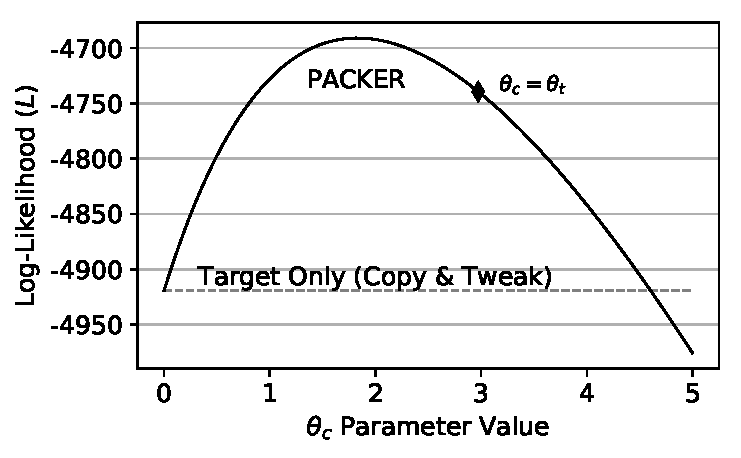
\includegraphics[width=\textwidth]{figs/packer-loglike.pdf}    
      \caption{PACKER's fit as a function of its prioritization of
        within-category and between-category similarity (using the $\theta_c$
        parameter) . To facilitate comparison, PACKER's other parameters ($c$,
        $\theta_t$) were set to the best fitting values obtained for
        copy-and-tweak in Table \ref{table:global-model-fits}. The black diamond
        marker indicates the log-likelihood for the point where
        $\theta_c=\theta_t$. }
    \label{fig:packer-loglike}
    \end{center}
\end{figure}


\subsection{Individual Differences}
\label{section:individual-diffs}

As noted in Experiments 1 and 2, we observed a great deal of individual
differences in the types of categories that participants generated. Within each
condition, there were a wide variety of category types, such as row and column
categories (see Figures \ref{fig:e1-samples} and \ref{fig:e2-samples}). The
simulations reported above serve to evaluate the models while considering the
entire dataset, but a secondary goal of any formal account should be to provide
some explanation of how different profiles of performance emerge. Many of the
individual generation profiles we observed can be described with the models
simply by tuning the model's parameters in a principled manner. In this section,
we describe more specifically how the most frequently observed profiles can be
realized.

By manual inspection, it is evident that the most common profiles of generation
consist of: (A) a tightly-distributed `cluster' of examples, (B) `row'- and
`column'-like arrangements (varying widely along one dimension but not the
other), and (C) a `corners' arrangement with examples placed into disparate
corners of the space. These four profiles are distinct in terms of the
distribution of the generated category along each dimension: Whereas the cluster
profile is tightly distributed along both dimensions, the row and column
profiles are tightly distributed along just one dimension. Finally, the corners
profile is widely distributed along both dimensions.

In the framework proposed by PACKER, the cluster and corners profiles arise
based on different prioritization of within-category similarity versus
between-category contrast, and the row and column profiles arise based on the
prioritization of each dimension in the computation of similarity. For example,
in the cluster profile, there is a high degree of within-category similarity
along both dimensions, whereas in the corners profile there is minimal
within-category similarity. Thus, PACKER's proposal is that these individual
differences arise as a result of different priorities: While the tight cluster
configuration can be considered PACKER's `default' mode (as it maximizes
within-category similarity), the corners profile can be produced when
between-category contrast is put at a higher priority (i.e., $\theta_c > \theta_t$).

Likewise, in the row and column profiles, there is a large degree of
within-category similarity along one dimension but not the other. These
differences likely arise due to a differential focus on one dimension over
another, and thus they can be produced by changes to PACKER's attention weights,
$w_1$ and $w_2$ (see Equation \ref{eq:similarity}). Traditionally, the attention
weights in exemplar models are thought to reflect the diagnostic value of each
dimension towards classifying the known category members
\citep{nosofsky1984choice,nosofsky1986attention,kruschke1992alcove}, but within
a generation context the weights specify the importance of within- and
between-category similarity along each dimension. For example, if all of
attention is allocated along the X-axis ($w_1=1$ and $w_2=0$), similarity along
the Y-axis no longer influences performance. As a result, PACKER will create
categories that are more widely distributed along the Y-axis, as similarity is
not taken into account along that dimension. As a general principle,
differentially weighting one dimension will result in the generation of
categories that are more widely distributed along the ignored dimension,
conforming to a row- or column-like arrangement. See Figure
\ref{fig:packer-attention} for a depiction of how attention influences PACKER's
performance.

\begin{figure}
    \begin{center} \inputpgf{figs/}{packer-attention-examples.pgf}
    \caption{PACKER generation of a category `B' example, following exposure to
one member of category `A' and one member of category `B'. Predictions are shown
for different attention settings: {\em (a)} Increased weighting of the X-axis.
{\em (b)} Increased weighting of the Y-axis. {\em (c)} Uniform weighting
(identical to Figure \ref{fig:packer-examples}).}
    \label{fig:packer-attention}
    \end{center}
\end{figure}

As in PACKER, changes in the parameter settings of the copy-and-tweak model can
also be used to produce different patterns of generation. Indeed, as
copy-and-tweak is simply a special case of the PACKER model, the attention
weights operate exactly as described above to produce row- and column-like
categories. However, because the model is not influenced by category contrast,
it is biased toward generating tightly clustered categories, as new items are
always most likely to be generated near known examples of the target category.
Thus, the lack of a contrast mechanism prevents the model from explaining why
some individuals widely distribute their categories to the corners of the space.

For both the hierarchical Bayesian and the representativeness models, the prior
domain covariance matrix $\Sigma_0$ can be used to explain the generation of
row-like and column-like categories. This covariance matrix specifies the amount
of variance assumed along each dimension (as well as the dimensional
correlations) across the domain of categories. The covariance matrix for a newly
generated category, $\Sigma_B$, is based on the assumed $\Sigma_0$ as well as
the distributions of previously learned categories (see Appendix
\ref{ap:hsampling-definition}). Thus, the importance of each feature can be
coded into $\Sigma_0$ to alter the dimensional variance of generated categories.
Because the hierarchical Bayesian model possesses no mechanism to account for
category contrast, the model is most likely to generate new items that are
similar to known examples of the target category with no regard for how
different it is to the contrast category. However, the representativeness model
predicts that new exemplars should provide more relative evidence to the `Beta'
category, accounting for the tendency of row-like and column-like profiles
occupying the edge of the feature space.

While the copy-and-tweak and hierarchical Bayesian models possess mechanisms to
explain row- and column-like categories, they cannot easily explain why some
individuals widely distribute their generated categories into disparate corners
of the space. This, however, reveals a more general limitation: According to the
copy-and-tweak and hierarchical Bayesian models, the distributional structure of
generated categories is {\em independent} of their location within the domain.
For example, although the copy-and-tweak or hierarchical Bayesian models can be
parameterized to generate row- or column-like categories, there is no mechanism
in place to ensure that what is generated will be distinct from what is already
known. In the next subsection, we explore this prediction through an analysis of
the interdependence between distributional structure and location in category
generation.

\subsection{Category Location vs. Distributional Structure}
\label{section:individual-diff}
As noted above, while all three models make clear claims about the internal
structure of generated categories, the copy-and-tweak and hierarchical Bayesian
models do not make any claims about how generated categories should differ from
what is already known. However, as we observed in the results of Experiment 2,
the distributional structure of a category is not always independent of its
location within the domain. To demonstrate this point in more depth, we computed
the X- and Y- axis ranges of every participant-generated category. Taking the
difference between these values ($X-Y$) produces a measure of each category's
orientation in the space: positive difference scores correspond to categories
with more X-axis range (horizontally aligned, `Row' categories), whereas
negative difference scores indicate the opposite (vertically aligned, `Column'
categories). Neutral differences scores indicate there was an equal amount of X-
and Y-axis range, which can be produced by a number of different category types
(`Clusters', `Corners', etc; see Figures \ref{fig:e1-samples} and
\ref{fig:e2-samples}). By plotting, for each possible stimulus, the difference
scores of categories it was generated within, we can relate the distributional
structure of generated categories to their location within the domain.

However, because many stimuli were infrequently generated (such items near
members of the `Alpha' category), we cannot simply compute the empirical average
of the difference scores, as infrequently generated stimuli would be likely to
show artificially strong differences. Instead, we used a Bayesian analysis to
estimate the mean $\mu_x$ on the assumption that the scores $x$ for each
stimulus are normally distributed with an unknown mean and unknown standard
deviation. The conjugate Normal-Inverse Gamma distribution provides a
straightforward method for this estimation:


\begin{equation} \mu_x = \dfrac { \nu_0 \mu_0 + \sum{x} } { \nu_0 + n }
\label{eq:rangediff-bayes}
\end{equation} \ where $\mu_0$ is the prior mean, $\nu_0$ is a prior scale
parameter (controlling the weighting of the $\mu_0$), and $n$ is the number of
categories in which the stimulus was a member (i.e., the number of scores in
$x$). The default assumption is that there is an equal amount of range along the
X- and Y-axes, and so we set $\mu_0 = 0$. Likewise, to give a moderate amount of
weighting to the prior mean we set $\nu_0 = 1$, though the results are robust to
a range of values. Within this approach, the resulting aggregation is a
trade-off between the number of generations and the strength of the range
difference within each generated category. Infrequently generated stimuli, as
well as those with mixed positive and negative scores, are given neutral
difference scores.

\begin{figure}[p]
    \begin{center} 
      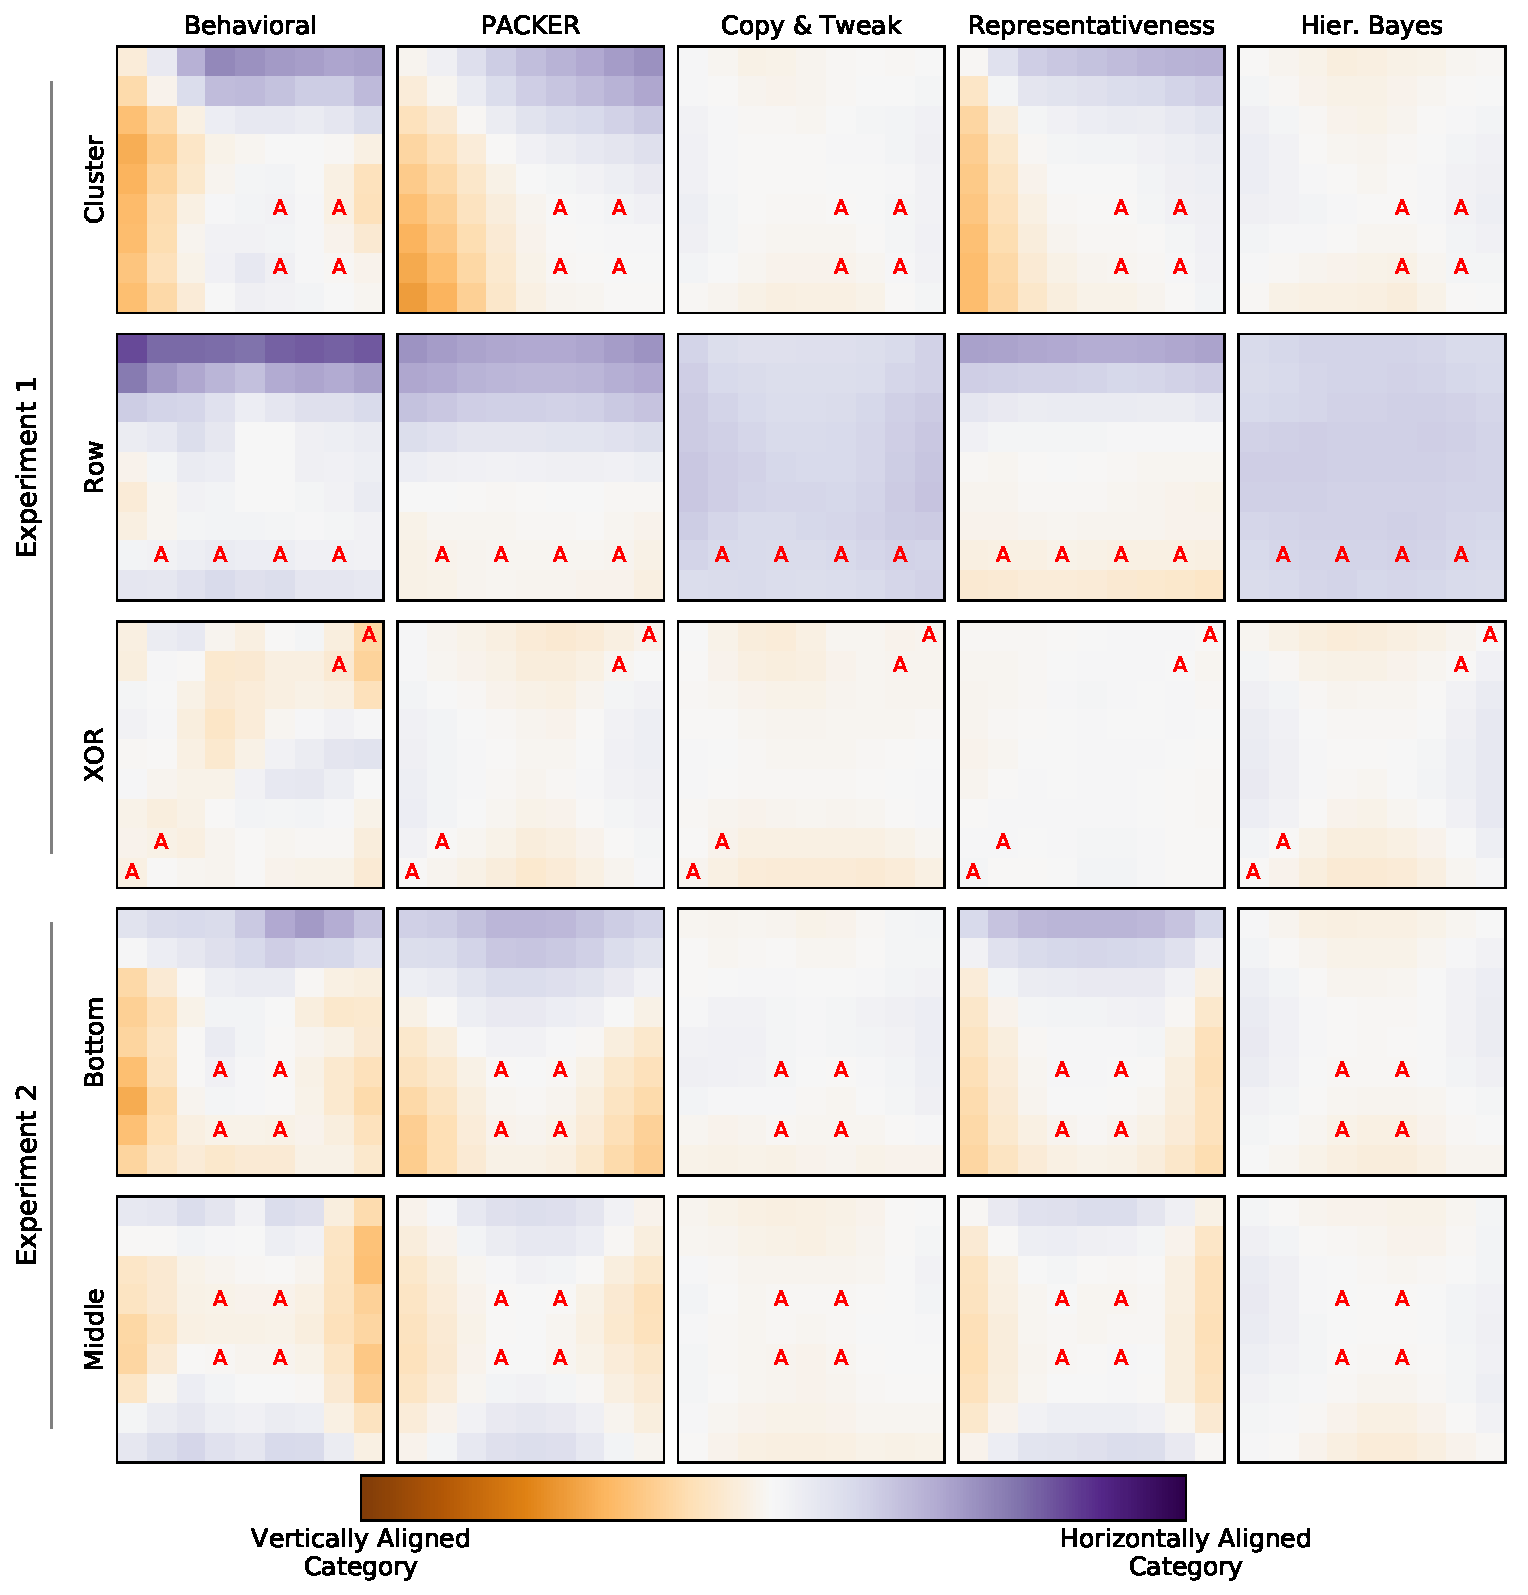
\includegraphics[width=\textwidth]{figs/range-diff-gradients.pdf}
      \caption{Behavioral and simulated range difference gradients. Each panel
        shows, for each stimulus, the dimensional orientation of the categories
        it was generated into: vertically aligned `columns' (orange) versus
        horizontally aligned `rows' (purple).}
      \label{fig:range-diff-gradients}
    \end{center}
\end{figure}

The results of our analysis are shown in Figure \ref{fig:range-diff-gradients}
for the experiment and model results\footnote{Prior to plotting, data were also
processed using a Gaussian filter with $\sigma = 0.8$.}. The left-most column of
Figure \ref{fig:range-diff-gradients} displays the effect of category location
and contrast on the distributional structure of the category generated by
participants. These data reveal strong and consistent patterns across all the
conditions we tested in Experiments 1 and 2: Generated categories are more
tightly distributed along the axis in which they are distinct. For example, in
the `Cluster' condition, exemplars in the bottom-left of the space are more
often generated into vertically aligned categories, and exemplars in the
top-right are more often generated into horizontally aligned categories.
Similarly, in the `Bottom' and `Middle' conditions, horizontally aligned
categories are generated above and below the experimenter-defined categories,
while vertically-aligned categories are generated to the sides. In the `Row'
condition, most categories are horizontally aligned, and lie along the upper
areas of the space. There are no strong range difference patterns in the XOR
condition.

These patterns of performance clearly depict the interdependence between the
distributional structure and location of generated concepts. Our results can be
interpreted in terms of local minimization of between-category similarity: By
distributing the generated category away from members of the
experimenter-defined category, participants may increase the degree of
between-category distance without drastically altering the degree of
within-category similarity.

To explore how well the PACKER, copy-and-tweak, representativeness, and
hierarchical Bayesian models explain our findings, we conducted simulations
using an individual-differences approach. As noted in Section
\ref{section:individual-diffs}, row- and column-like categories can be produced
by each model through changes to the weighting of each dimension. Given this
information, we may use the models to simulate each participant's generation
separately, with the importance of each dimension set according to the relative
range of the participant's generated category along each dimension.

In the PACKER and copy-and-tweak models, the attention weights, $w$, specify the
importance of each dimension in the computation of similarity. While there exist
methods to find the optimal attention weighting scheme given a classification
\citep[see][]{vanpaemel2012using}, for simplicity we assume that the `Alpha' and
`Beta' categories are distinct along dimensions that the `Beta' exemplars do
not vary on. In this case, the weighting for a given participant can be computed
as:

\begin{equation} w_k = \dfrac {\exp{ \{ -\theta_w \cdot\text{range}(k)} \} } {
\sum_k {\exp{ \{ -\theta_w \cdot\text{range}(k)} \} } }
\label{eq:range-weight}
\end{equation}
% 
where $\theta_w$ is a free parameter controlling how differences in range
correspond to differences in weights (functioning similarly to the $\theta$
parameter in each of the models), and $\text{range}(k)$ is the range of examples
generated by the participant along dimension $k$. We used $\theta_w = 1.5$ in
our simulations, though the results are robust and similar for other $\theta_w$
values. The resulting $w$ values are thus inversely proportional to the range of
generated categories along each dimension, with less range corresponding to
greater weighting.

Unlike the PACKER and copy-and-tweak models, the representativeness and
hierarchical Bayesian model's dimensional variances correspond to the assumed
variance of generated categories along each dimension (rather than the inverse
of the variance). Thus, a different transformation is appropriate for
incorporating the weights computed in Equation \ref{eq:range-weight}. For the
hierarchical Bayesian model, we computed the dimensional variances according to:
$\lambda (1-w_k) 2$, where $\lambda$ is a free parameter specifying the overall
assumed variance of the domain, and $2$ corresponds to the number of dimensions
in our experiments\footnote{This calculation applies only in two-dimensional
  domains, where $w_2 = 1-w_1$.}. Under this approach, evenly distributed
weights correspond to an assumed variance of $\lambda$. Likewise, larger values
of $w$, which are produced when the generated category is tightly distributed
along one dimension, correspond to smaller assumed variances.

Each model was used to simulate each participant's generation independently,
with the importance of each dimension set according to the participant's
generated category. The other free parameters within each model were set as in
Table \ref{table:global-model-fits}. Every participant's generation was
simulated 2,000 times; given the 305 participants tested across the two
experiments, each model generated 610,000 categories in total. For comparison
with our behavioral results, we then computed the range difference gradient
identically as with the behavioral data. The results are shown in Figure
\ref{fig:range-diff-gradients}.

As in the more traditional model evaluation analysis described above, the
contrast models (i.e., PACKER and the representativeness model) provided a much
closer match to our behavioral results than the copy-and-tweak and hierarchical
Bayesian models. In all conditions, the contrast models distribute categories
similarly to the behavioral data: Horizontally-aligned categories tend to be
placed above and below members of the experimenter-defined category, and
vertically-aligned categories tend to be placed to the sides. Conversely,
because the copy-and-tweak and hierarchical Bayesian models are insensitive to
category contrast, these models do not produce any systematic patterns of
association between category location and distributional structure. The sole
exception is within the `Row' condition of Experiment 1, in which the majority
of participants generated a `Row'-like category, widely distributed along the
X-axis but not the Y-axis. In these cases, both models are initialized with
weights that produce Row categories, but because category contrast is not
considered, categories are uniformly generated across the entire domain, rather
than concentrated within the upper-regions as observed behaviorally.

%Experiment 3 starts here
\section{Experiment 3}

Experiments 1 and 2 clearly establish the importance of contrast in category
generation. Follow-up model-based analyses illustrated that both contrast models
account for participant performance better than models that do not take into
account contrast. We also found more support for contrast as representativeness
hypothesis over contrast as exemplar dissimilarity hypothesis.

Although category generation is an intriguing aspect of human cognition, it has
played a relatively limited role in the broader categorization literature. To
establish that contrast plays a broader role in categorization, we conducted a
traditional category learning study. In it, participants learned two categories,
where the categories learned by each participant in Experiment 3 was yoked to
the `Alpha' shown and `Beta' generated by each participant in Experiment 2. Our goal
is to investigate whether model performance (in generating categories) is
consistent with human performance (in learning those categories). Specifically, if contrast plays a broader role in categorization, then `Beta' categories rated as "better" according
to the contrast models should be easier for participants to learn.
%\footnote{It is possible to adjust the present models of category generation such that they can make category learning predictions. However, such an adjustment makes the strong assumption that the very same processes governing category generation also apply to category learning. Taking this approach would fall outside the scope of the current investigation.} 
\subsection{Participants, Materials, and Procedure}

Experiment 2 recruited 122 participants who each generated one set of four `Alpha'
and four `Beta' category exemplars. Experiment 3 recruited the same number of
participants.

Participants observed four blocks of eight trials. Each trial began with the
presentation of a fixation cross for 500 ms. This was followed by the
presentation of one exemplar randomly sampled without replacement from the
unique category set. Participants were tasked with assigning the presented
exemplar to either the `Alpha' or `Beta' category with no time limit imposed.
Feedback was automatically displayed for 2500 ms after each response.

\subsection{Results and Analysis}

Among the 122 originally generated category sets were 102 unique sets (i.e.,
they contained a unique collection of `Alpha' and `Beta' exemplars). Consequently,
for our subsequent analyses for this experiment we only use data from the first
102 participants that were presented with a unique category set.

Overall accuracy of the participants was high, with a mean error rate of $.19$
($SD = .19$). Aggregated error rates for each block are presented in Figure
\ref{fig:learningcurve}.

\begin{figure}
    \begin{center}
    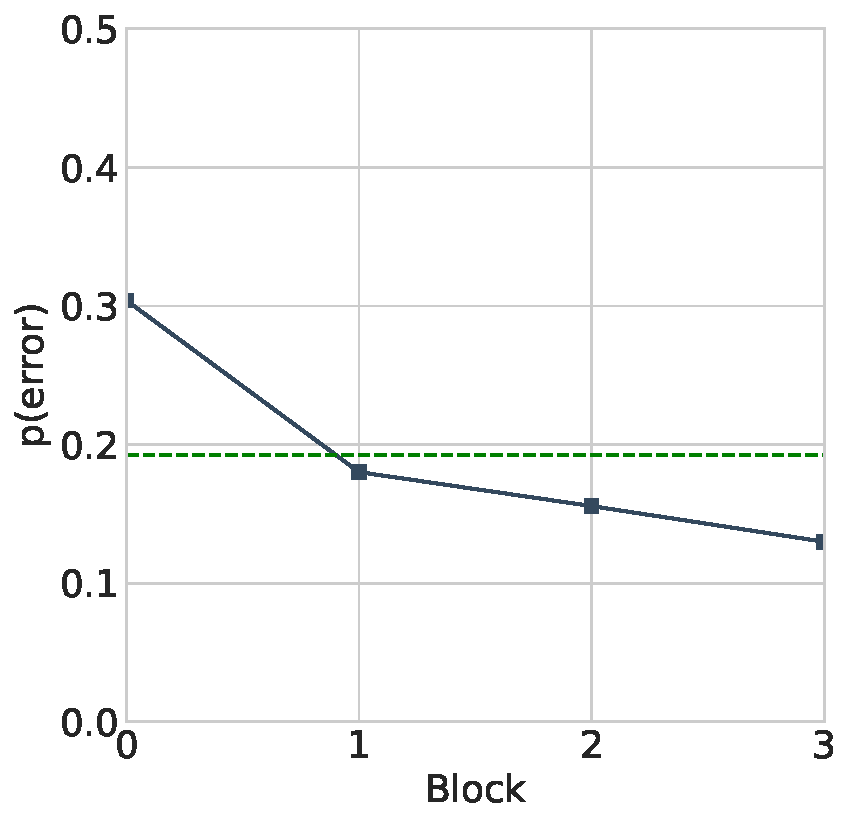
\includegraphics[width=\textwidth/2]{figs/e3-learningcurve.pdf}
    \caption{Average error rate for each successive block. Green discontinuous
line represents the overall mean error rate.}
    \label{fig:learningcurve}
    \end{center}
\end{figure}

In order to analyze the consistency between model and human performance, we
optimized each model such that the Pearson correlation between the model's
negative log-likelihood of generating each unique category set and the
participant's error in learning that category set is maximized. As with the
analysis in Section \ref{section:individual-diff}, we simulated the weighting of
each dimension independently depending on the generated categories.

The greatest correlations were observed when fitting the contrast models.
Specifically, PACKER correlated with human performance with
$r = .65, 95\%\,CI\, [.48,.78]$, and the representativeness
model correlated with human performance with $r = .59, 95\%\,CI\,[.40, .73]$\footnote{Confidence intervals were obtained using a bootstrap
  method with 1000 bootstrap samples.}.
Copy-and-tweak yielded a correlation of $r = .45, 95\%\,CI\,[.28, .62]$ and the
hierarchical Bayesian model yielded a similar correlation of
$r = .46, 95\%\,CI\, [.30, .62]$. These results are graphically presented in Figure
\ref{fig:perror_corr}.

\begin{figure}
    \begin{center}
    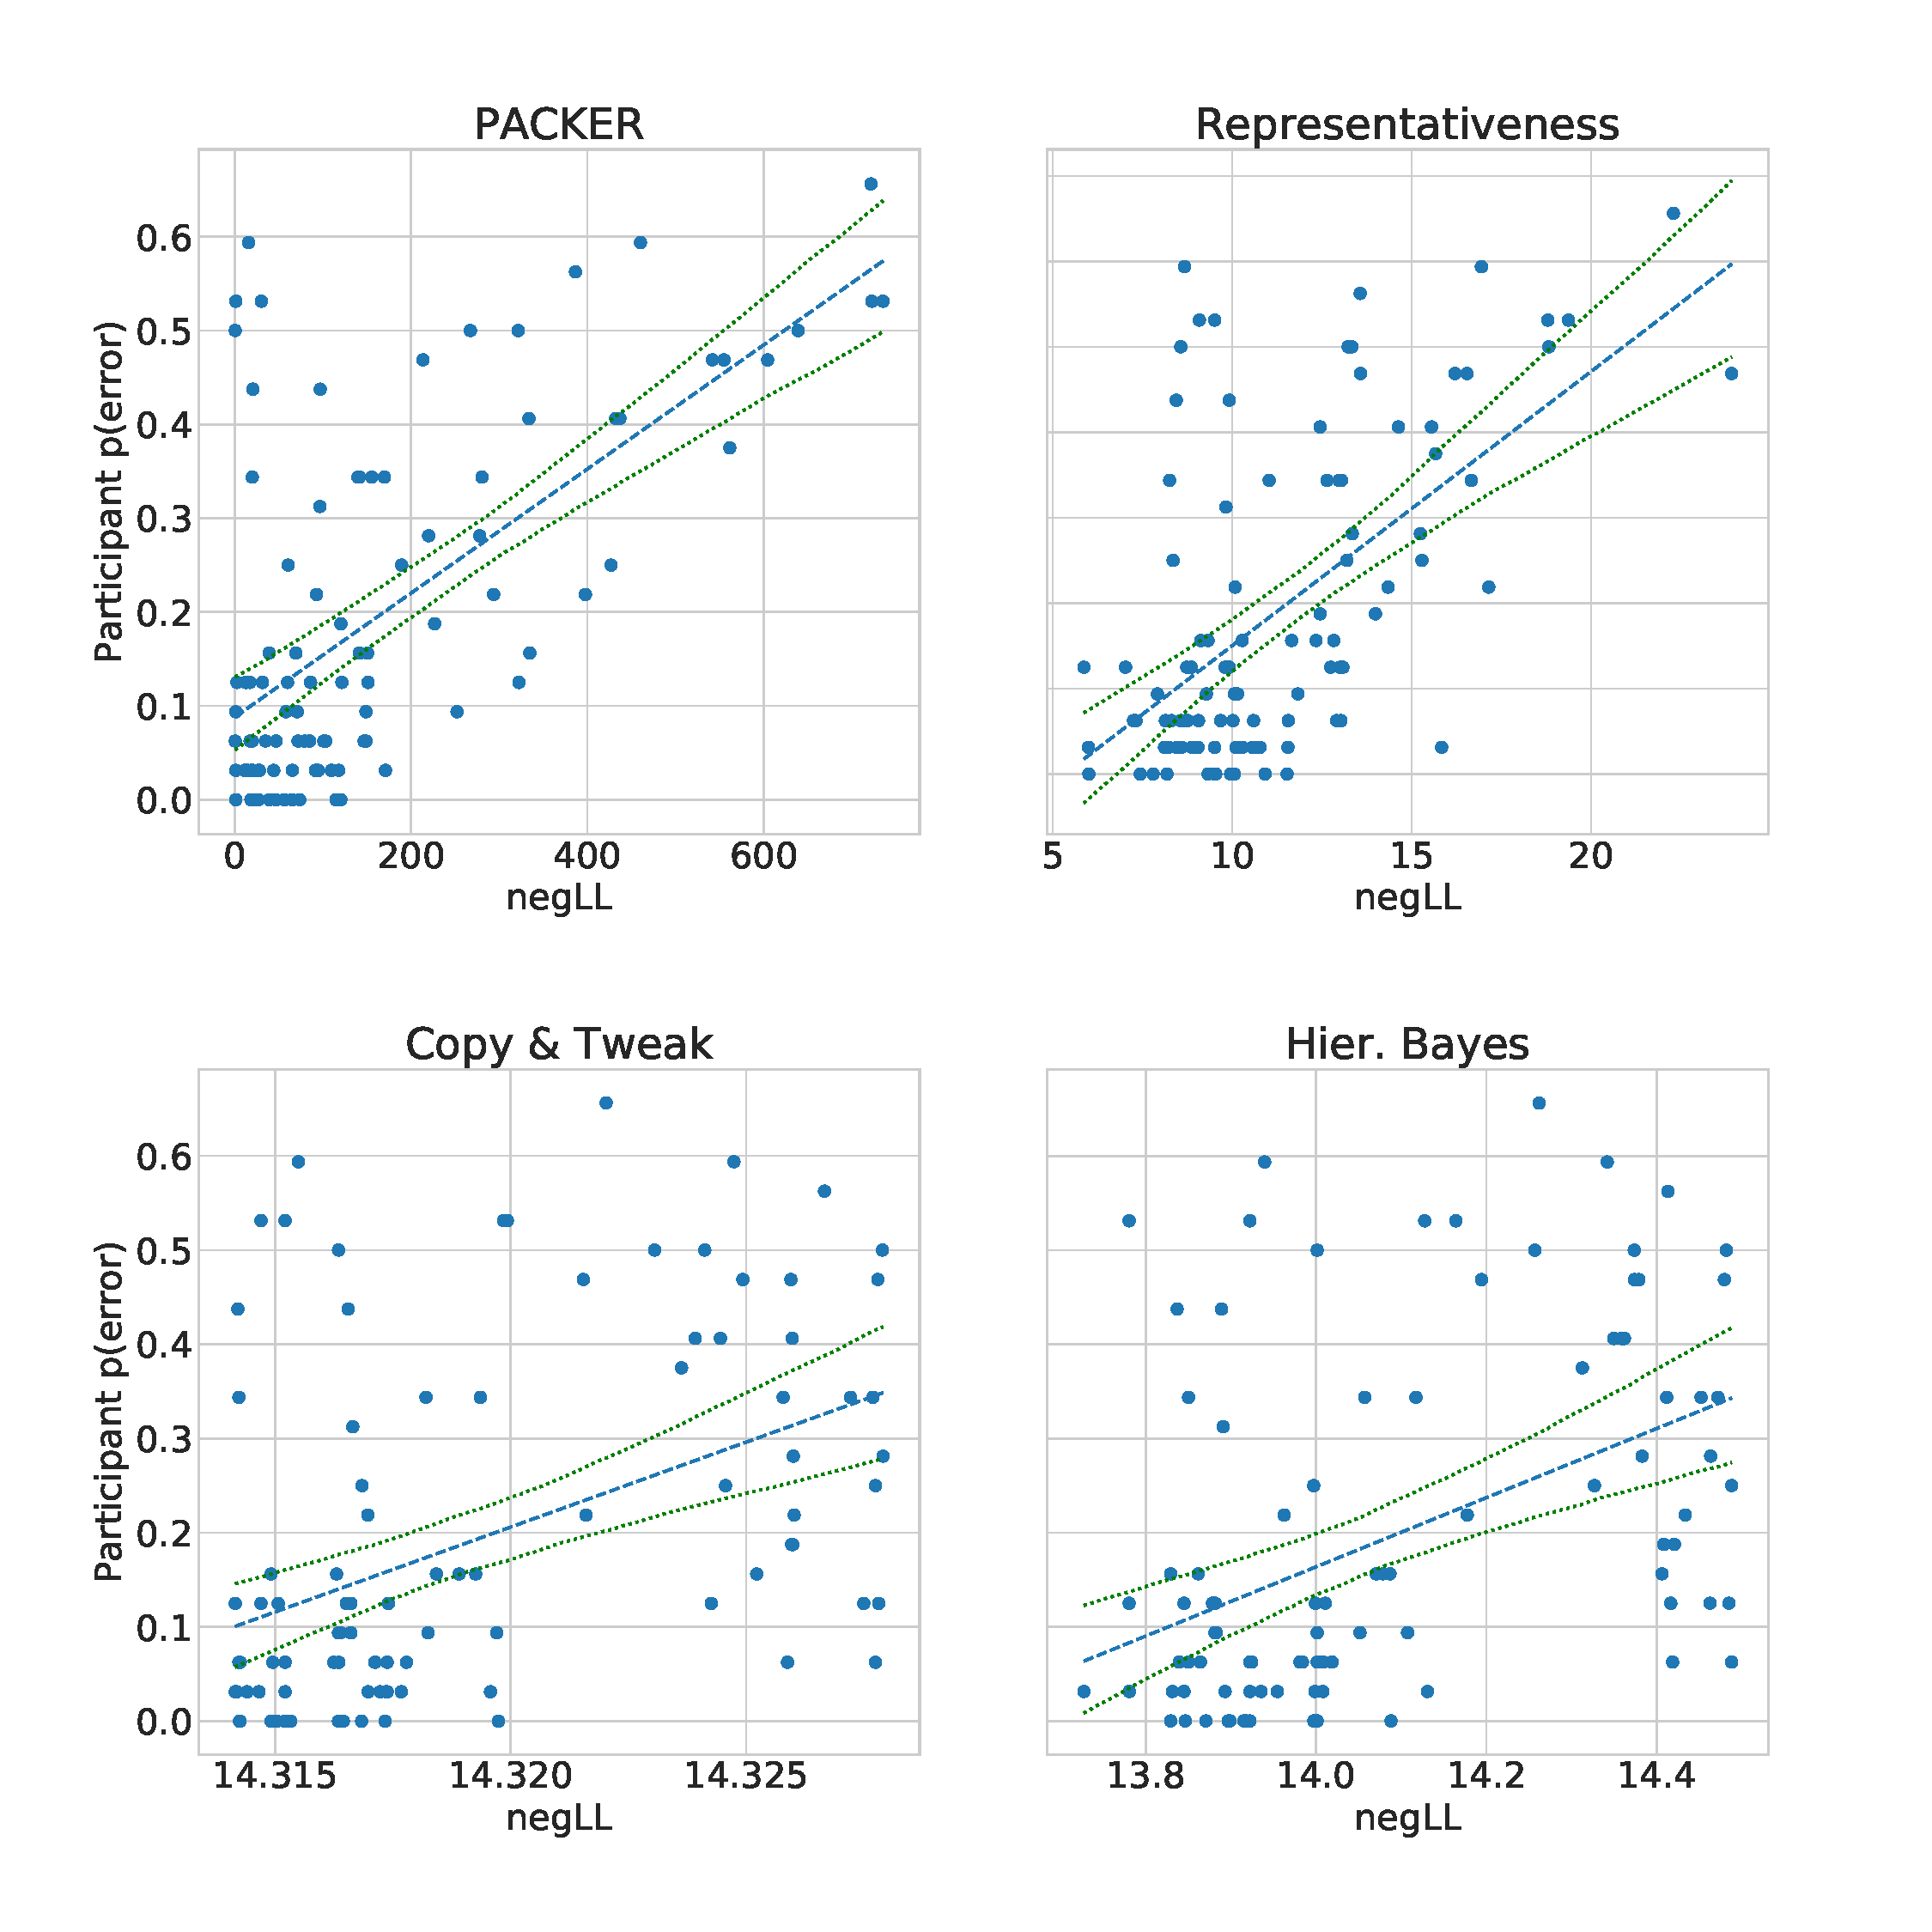
\includegraphics[width=\textwidth]{figs/modelvspptp.pdf}
    \caption{Scatterplots indicating the correlations between observed
      participant error and model fit. Blue discontinuous line are best-fit
      lines. Green discontinuous lines indicate boundaries generated by the 95\%
      CI around the fitted correlations. }
    \label{fig:perror_corr}
    \end{center}
\end{figure}

To emphasize the strong influence of contrast in maximizing the association
between category generation and category learning, we computed the correlations
over wide range of $\theta_{contrast}$ values, with the other parameter values
of PACKER held constant at their optimized levels. As presented in Figure
\ref{fig:packer-corr}, the correlation quickly increases with increasing weight
on contrast, reaching a plateau above values of around 4.0.

\begin{figure}
    \begin{center}
    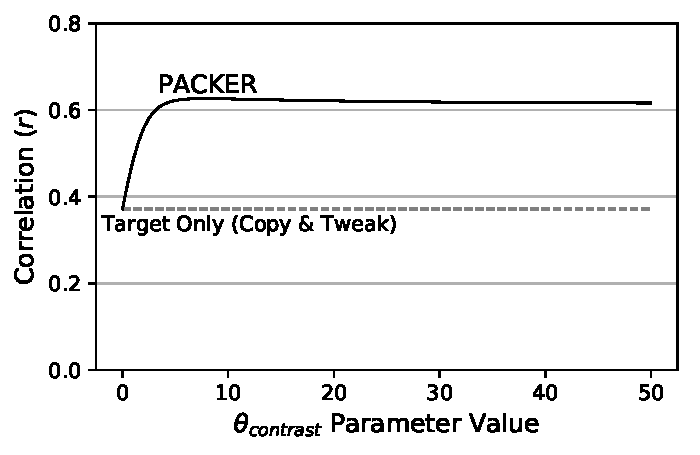
\includegraphics[width=0.8\textwidth]{figs/packer-corr.pdf}
    \caption{Correlation between PACKER's fit and participant error as a
function of the $\theta_{contrast}$ parameter. To facilitate comparison,
PACKER's other parameters ($c$, $\theta_{target}$) were set to the best fitting
values obtained for copy-and-tweak in Table \ref{table:global-model-fits}. Grey
dashed line represents the correlation between Copy \& Tweak's fit and
participant error.}
    \label{fig:packer-corr}
    \end{center}
\end{figure}

\section{General Discussion}
The sensory impression of every stimulus and event is unique. Grouping distinct patterns of sensory information into categories is a fundamental task solved by the mind. Most work has focused on how people learn new categories that are provided to them through unlabeled, partially labeled, or fully labeled examples. How were these categories first determined? Some natural categories are likely to be the result of regularities in the dynamics of our environment. But, these are only a subset of the categories that people learn. Other categories, such as tools and ideas, were generated by people over time. What basic principles underlie how people generate categories?

While the bulk of prior research on categorization has focused on the classic
finding that generated concepts tend to be distributionally similar to known
concepts, there has been little work addressing the role of contrast in category
generation: How is it that people are able to create something {\em different}
from what is already known? We developed two novel models, each incorporating a
different conceptualization of category contrast. One model is PACKER, which is
an exemplar-based model that formally specifies the role of contrast in
generation as exemplar dissimilarity. Specifically, the model proposes that
categories are represented as exemplars in a multidimensional psychological
space, and generation is constrained both by within-category and
between-category similarity: Exemplars belonging to the same category should be
similar to one another, and exemplars belonging to different categories should
not be similar to one another. The second model is a novel hierarchical Bayesian
model with a representativeness mechanism. This model generates exemplars that
are more representative of (i.e., has greater relative evidence from) the novel
category compared to the learned category.

We reported two experiments demonstrating systematic effects of category
contrast in category generation. Members of participant-generated categories
tended to be highly dissimilar from members of previously-learned categories,
and were usually more similar to one another than to members of other
categories. We also observed broad interdependence between the distributional
structure (feature variance, correlation) and physical instantiation (location
within the stimulus space) of generated categories: In Experiment 2, we found
that the unoccupied regions of the domain influenced the distributional
structure of categories, and in both experiments we observed that participants
distributed their generated categories to increase contrast with what was
already known.

We conducted simulations comparing the contrast models' account of our results
to the classical proposals for category generation: a ``copy-and-tweak'' model
(realized as a variant of PACKER with no sensitivity to category contrast), and
a hierarchical Bayesian model designed to explain the classic distributional
similarity effect. In all simulations, we found that the contrast models
captured a previously unexplained and unexplored aspect of human category
generation. In particular, by measuring PACKER's fit as a function of its
prioritization of within- and between-category similarity, we observed that
considering either constraint exclusively results in a relatively low-quality
account. Instead, PACKER's best results were obtained when both constraints are
considered, indicating that human learners do not generate novel concepts
exclusively on the basis of within-category similarity or between
class-contrast. This finding mirrors our behavioral results and demonstrates
that both constraints influence generation when explained with an exemplar
model. Ultimately, our category generation data were best explained by the
representativeness model. The exact nature of its superiority over the other
models is still not yet clear. However, as we explore in a later section, it is
likely that the representativeness mechanism itself (i.e., independent of the
hierarchical Bayesian foundation) captures a core aspect of both category
generation and category learning.

\subsection{Finding Contrast Effects in Prior Work}

Although existing accounts of category generation broadly overlook the role of
category contrast in determining what is novel versus familiar, it was
implicitly assumed that learners in previous experiments were {\em successful}
in creating new categories. Thus, if contrast plays a robust role in category
genration, its effects should be discernable within the experimental results of
these studies. To provide a test of the influence of category contrast within
existing data, we conducted a novel analysis of Experiment 3 from
\cite{jern2013probabilistic}.\footnote{Although \cite{jern2013probabilistic}
reported four experiments, we focus on Experiment 3 because their first two
experiments tested generation of items into known categories, and their fourth
experiment was identical to Experiment 3 but with a restricted generation
space.}

Participants in their experiment were exposed to members of two
experimenter-defined categories of `crystals' varying in hue, saturation, and
size. Each category possessed a unique hue, but varied in saturation and size:
In the `Positive' condition, there was a positive correlation between these
features (i.e., larger sized crystals were more saturated), and in the
`Negative' condition this relation was reversed. In the `Neutral' condition,
there was no correlation between saturation and size. After learning about the
categories from each condition, participants were asked to generate six
exemplars belonging to a novel class. As noted above,
\cite{jern2013probabilistic} found that the generated categories tended to
follow the distributional properties of the experimenter-defined categories:
Generated categories were tightly distributed along the hue feature, and
possessed the same saturation-size correlations as in the learned categories.
\cite{jern2013probabilistic}, however, did not analyze or discuss how the
generated categories {\em differed} from the experimenter-defined categories.

Because each experimenter-defined category in the \cite{jern2013probabilistic}
experiment possessed a distinct hue shared by all members of the category, it is
sensible that participants might generate a category with a hue distinct from
the experimenter-provided categories. If category generation were influenced by
category contrast in this way, the hues of generated categories should be
systematically different from those of the experimenter-defined categories.
Unfortunately, stimulus hue was encoded and presented in the
Hue-Saturation-Value (HSV) color space, which is device-dependent and not
perceptually normed such that perceived color similarity corresponds to
proximity in the color space (as opposed to a color space such as CIELAB that is
device-independent and equidistant sets of points correspond to pairs of colors
that have the same perceptual similarity; \citealp{wyszecki1967}). Further, they
did not calibrate their monitor, and so we cannot know the precise colors
presented to participants. As \cite{jern2013probabilistic} were interested in
relations between the saturation and length of examples in generated into novel
categories, these issues do not undercut their analyses and results. However,
these issues pose a significant challenge to evaluating contrast between the
experimenter-defined and participant-generated categories along the hue
dimension. It is plausible that two uncalibrated monitors could display the same
HSV color and the colors be perceived in different color categories (especially
for color boundaries that vary over lightness, such as the yellow-brown
boundary).

Although we cannot know the precise colors that were displayed or perceived, we
can still analyze their results from a coarse perspective to see whether there
is preliminary support for contrast. To do so, we binned all possible hues into
one of eight uniformly-spaced color groups: \{{\em Red}: $0-0.063$, $0.938-1$,
{\em Yellow}: $0.063-0.188$, {\em Yellow-Green}: $0.188-0.313$, {\em
Green-Teal}: $0.313-0.438$, {\em Teal}: $0.438-0.563$, {\em Teal-Blue}:
$0.563-0.688$, {\em Purple}: $0.688-0.813$, {\em Pink}: $0.813-0.938$\}. In the
\cite{jern2013probabilistic} experiment, the hue of each experimenter-defined
category was selected from one of six possible values, each of which falls into
one of the color groups above (two color groups were not used as a possible hue
for the experimenter-defined categories). By categorizing the
participant-generated crystals likewise, we can obtain a broad measure of
category contrast by determining the proportion of participant-generated
crystals that fall into the same groups as the experimenter-defined categories:
If contrast influences the hues of the generated categories, we should observe
minimal overlap between in the color groupings.



\begin{figure}
    \begin{center} \inputpgf{figs/}{jk13-huecontrast.pgf}
        \caption{Analysis of data from \cite{jern2013probabilistic}, Experiment
3. Plotted is the number of generated items that share a color group with one of
the experimenter-defined classes. The ``Expected'' data follows a Binomial
distribution with $p = 2/8 = 1/4$, given there were two experimenter-defined
classes, and eight color groups.}
        \label{fig:jk13-huecontrast}
    \end{center}
\end{figure}

These data, shown in Figure \ref{fig:jk13-huecontrast}, reveal a clear pattern:
The majority of participants in each condition ($n = 22$) generated categories
possessing entirely distinct hues; with 0/6 exemplars sharing a hue with the
experimenter-defined categories. These results can be compared to the
predictions of a Binomial model, which proposes that participants generate hues
at random. That is, if hue selection is not systematic, the probability that any
given example will lie in the same color group as an experimenter-defined
category is given by a Binomial distribution with $p = 2/8=1/4$, as there were
two experimenter-defined categories and eight possible color groups. Chi-square
goodness-of-fit tests reveal that the observed distribution in each condition is
highly inconsistent with the hues being chosen at random, all
$\chi^2(6,N=22)>200$, $p < .001$. Participants tended to generate items that were
perceptually distinct from the categories they had learned, and were less likely
to generate hues possessed by members of the experimenter-defined categories.

It is possible, however, that this data can be explained by a process that does
not involve contrast. Specifically, since participants were trained on exemplars
that share the same hue within a category, it is plausible that they generate
exemplars that all share a common hue. If this were the case, given a $6/8 = .75$
probability that a hue distinct from the experimenter-defined categories is
selected, there is a corresponding $.75$ probability (or about 17 out of 22
participants) that the generated category will have no exemplars that share a
hue with any  of the experimenter-defined categories. In addition, that there is
a $2/8 = .25$ probability (about 6 out of 22 participants) that the generated
category will have all six exemplars that share a hue with any of the
experimenter-defined categories. This prediction of regularity across categories
is much closer to the data than the prediction from a Binomial model and does
not require any mechanism of category contrast.

However, upon analyzing the consistency of hues in the generated categories, it
is clear that participants do not generally produce categories with entirely
similar hues across all exemplars. Specifically, only 55\%  of all generated
categories comprised exemplars with a common hue. Consequently, the assumption
of regularity across categories may be inappropriate for this data set, leaving
the contrast-based explanation as the most plausible for our purposes.

Re-analyzing the results from \cite{jern2013probabilistic} provides some
corroborating support for contrast playing a role in category generation. Taken
alongside the analyses reported by \cite{jern2013probabilistic}, our analysis
suggests that generated categories tend to be distinct from {\em and}
distributionally similar to what is already known. However, it is worth noting
that our analysis is still limited: The color groups defined above are
imprecise, and it is not clear that our color grouping is consistent with the
psychological color boundaries perceived by participants. While we did obtain
similar results using a variety of alternative groupings, the hue dimension used
in the \cite{jern2013probabilistic} study does not lend itself straightforwardly
to the computation of similarities, and thus we cannot be certain of whether our
coding accurately approximates the psychological space of the stimuli. This
precludes traditional applications of categorization models to their data as it
is usually necessary to encode objects in psychological space in order to
accurately determine the similarity between objects. By consequence, although
these results likely indicate that contrast exerts {\em some} influence, they do
not precisely describe the nature of that influence. 

\subsection{Similarity and Contrast in Cognition}
The proposal that category contrast is a primary constraint in categorization is, in some ways, entirely commonsense. For categories to be useful, they should not all be identical, or in other words, they should be different. Thus, a newly generated category should be different than pre-existing categories. Beyond its role
in category generation specifically, category contrast is also of fundamental importance in
categorization more broadly. All other factors held constant, new categories are
easier to learn if they are dissimilar to members of other categories, and
knowledge of highly distinct categories is applied more accurately than that of
ill-defined categories \citep{ashby1994categorization,imai1965discriminability}.
Likewise, basic-level categories \citep{rosch1976basic} are thought to be
abstracted in order to maximize within-category similarity while minimizing
between-category similarity. Finally, the act of forming category
representations affects similarity judgments about category members and
nonmembers, with category members being viewed as more similar to one another
than members of other categories
\citep{goldstone1994influences,goldstone2001altering,goldstone1996isolated}.

Beyond categorization, one can find instances of the trade-off between within
and between-class similarity in linguistic categories over perceptual
dimensions. For example, \cite{regier2007} showed that the partitioning of color
categories reflects such a trade-off in a psychological space -- colors are
partitioned into groups with members that are viewed as highly similar to one
another yet distinct from other colors. A similar trade-off can be observed in
phoneme categories. Different exemplars of the same phoneme must be similar to
one another, while contrasting from other phonemes, such that a listener can
infer the appropriate phoneme. This pattern has been found and modeled in the
natural acoustics of American English vowels
\citep{feldman2013,hillenbrand1995}. As linguistic categories must have been
created at some point in human history, it is revealing that the constraints of
emulating distributional structure across categories and having categories
contrast from one another still bias human category generation today.

The dual forces of within-class similarity and between-class contrast influence
cognitive functions in a wide variety of domains. The PACKER model is notable in
that it explicitly interprets this trade-off within the domain of
categorization, and allows us to begin to understand the relatively understudied
processes involved in category generation through our more well-developed tools
for understanding human categorization.

\subsection{Implications for Creative Cognition}

Although the focus of this article has been to address the role of contrast in category generation and learning, our findings and approach have relevant implications
for research in creative cognition. A central focus of the creative cognition
approach has been to explain acts of creativity in terms of the mental
representations and processes that are commonly studied in cognitive psychology
and cognitive science \citep{finke1992creative,smith1995creative}. However,
unlike other fields in the study of cognition, creative cognition research
rarely employs quantitative models to evaluate the explanatory value of such
representations and processes. Our modeling results provide a concrete example
of how formal approaches may be used to gain insight into the nature of creative
cognition.

In addition to demonstrating the utility of formal modeling for studying
creative cognition, the contrast models here specifically offer an additional
interpretation of some of the field's most central findings. For example,
perhaps the most foundational principle from this literature concerns the
limiting influence of prior knowledge: Individuals create new categories
composed of features from existing classes, and what is created can be
influenced drastically through the introduction of cues or examples
\citep{marsh1999inadvertent,smith1993constraining}. In this paper, we have
identified another important aspect of the constraining influence of prior
knowledge: What is generated cannot be the same as what is already known.
Further, there is systematicity in how generated categories differ from prior
knowledge. The results of our simulations suggest that this conceptualization of
difference can be addressed in at least two different ways. Specifically,
simulations with PACKER demonstrate that the constraining influence of
difference is concisely explained in terms of a trade-off between
within-category similarity and between-category dissimilarity. Conversely, the
representativeness model shows that this influence can also be the result of
enhancing the representativeness of generated exemplars to their category.

PACKER may offer an additional interpretation of existing accounts of creative
generation. Most notably, a leading account within the creative cognition
literature, the Path of Least Resistance \citep{ward1994structured,ward1995s},
also explains generation in terms of an exemplar-based retrieval process. This
account was designed to explain the creative generation of natural categories
(e.g., new species of plants and animals) and as a result relies strongly on the
hierarchical organization of these categories: Individuals are thought to
retrieve an example of the higher-level category being generated (e.g.,
\textit{bird} may be retrieved from the category \textit{animal}), and then
systematically alter what was retrieved to make something new. As the PACKER
model does not assume knowledge is hierarchically organized \citep[this is true
of the exemplar view more broadly, see][]{murphy2016exemplar}, the model may be
viewed as a formal instantiation of the Path of Least Resistance for application
in a traditional artificial categorization domain (when there is no established
hierarchy of categories). PACKER's success in explaining generation within an
artificial domain motivates future work exploring the nature of category
contrast within a more naturalistic setting.

The broader study of creativity currently involves a wide breadth of different
approaches\citep[for a review see][]{kozbelt2010theories}, such as those based
on free association \citep{mednick1962associative} and conceptual combination
\citep{estes2002emergence,murphy1988comprehending}. In addition, recent work in
the machine learning literature has explored using neural networks to address
the overall problem of creative generation
\citep[e.g.,][]{goodfellow2014gan,ho2016gail,kingma2016,chen2016infogan}. In
contrast to these varied investigations, we reduced our focus by studying a
highly complex behavior (category generation) as it applies within a
well-established domain (artificial category learning). We hope that future work
incorporates and highlights the importance of contrast into theories of
creativity.

\subsection{Implications For Categorization}

Categorization research addresses the representations and processes that
underlie the learning and use of categories. Category learning tasks are
generally about figuring out which items belong to which category. Once learned,
categories are generally used to classify new stimuli and to make inferences
beyond the available information. Our work is fairly unique in that people learn
a single category through positive examples and then create another category
that would make sense in the domain. In other words, only one category is
provided to be learned and the use that is required of that category is to
generate a contrast category. Such scenarios have direct application to
real-world situations. For instance, consider being stranded in an unfamiliar
environment where you eat and get sick from a plant with certain features. In
avoiding such plants and seeking alternative sources of nutrition, it would
behoove you to imagine what features an edible, safe plant would possess (e.g.,
if the poisonous plant was bright red, perhaps a non-red plant would be safe to
consume). In the present studies, we have learned something about the form that
such expectations are likely to take. 

We can think of the category generation task in our studies as asking a person
to formulate an idea about what set of items in the domain are most
interestingly {\em not} members of the original category. To meet this
condition, the items must take some form of coherence that aligns with that of
the original category and some form of distinctiveness relative to the original
category. Reflecting the basic level of organization in natural categories, it
makes sense to generate a set of items that possess strong within-category
coherence (by importing or systematically transforming the internal structure of
the original category) as well as strong between-category differentiation (by
creating maximum contrast with the original category, be it through
exemplar-based dissimilarity or the maximization of exemplar-category
representativeness). In this sense one can see the patterns of performance in
the category generation task as recapitulating the order of semantic
organization.

The current work also suggests exciting directions for related investigations
into unsupervised categorization. While the unsupervised categorization
literature is primarily interested in the generation of categories within a set
of observed exemplars where no prior categories are learned, our category
generation studies are focused on the production of novel category exemplars
themselves. Despite this distinction, both types of categorization research are
ultimately interested in the question of how categories can be formed. The results
of our current work indicate that the formation of categories is constrained by
some measure of contrast. To our knowledge, this explicit investigation of
category contrast has not yet been attempted in the unsupervised categorization
literature. 

Interestingly, the unidimensional sort bias that is commonly observed in
unsupervised categorization
\citep{imai1965discriminability,milton2004influence,ahn1992two}, where
participants sort unlabelled family resemblance category exemplars by focusing
on a single feature, was not consistently observed in our tasks. In our
experiments we only observed this bias in the row condition of Experiment 1,
whereas in other conditions participants generated categories that typically
varied along both dimensions. This may be unsurprising at face value, since
participants in conditions other than the row condition were trained on a prior
category that varied on both dimensions. However, these results suggest that the
unidimensional sort bias is not universal to all types of category construction
-- or more specifically, the unidimensional bias may not apply when participants
need to generate categories with entirely new exemplars.

\subsection{Exemplar Dissimilarity and Representativeness in Categorization} 
Although both PACKER and the representativeness model perform better than the
classical models, they appear to be capturing fundamentally different aspects of
contrast in categorization. Specifically, while the representativeness model
excelled in predicting our category generation data, PACKER was the best-fitting
model in accounting for participant error in category learning. Given the
history of their development, this is perhaps not entirely surprising. PACKER
is implemented as an extension of the GCM, which was originally developed for (and
has been highly successful in) category learning \citep{nosofsky1986attention,
  nosofsky1994comparing}. Conversely, the representativeness mechanism was
conceived as a heuristic describing the relative extent to which an individual
observation is generated from some unobserved population
\citep{kahneman1972subjective,abbott16}. This generative nature of the
representativeness mechanism intuitively lends itself to the prediction of
category generation data. 

While the contrast models were born quite naturally out of the corresponding
classical models, it is worth considering if similar benefits in prediction
would be seen if the contrast mechanisms were applied to different classical
models. Although there is no clear way to adapt the exemplar dissimilarity
mechanism to the current hierarchical Bayesian model, it is a fairly
straightforward process applying the representativeness mechanism to an exemplar
model. Specifically, by treating the similarity measure (Equation
\ref{eq:similarity}) in the current implementation of copy-and-tweak as a
density estimate for the representativeness mechanism (Equation
\ref{eq:representativeness}), we gain a new model of representativeness that is
based on exemplar similarity instead of a multivariate Gaussian
likelihood.\footnote{An analogous implementation of the representativeness
  mechanism to PACKER results in both $\theta_c$ and $\theta_t$ adding to
  constant value that is independent of the similarity to contrast and target
  exemplars respectively. Consequently, it is formally equivalent to a
  copy-and-tweak model with representativeness.}

How well does a representativeness model that uses exemplar similarity to
represent the category’s density over features explain our experimental results?
We find that this model substantially outperforms its classical counterpart, but
not to the extent of PACKER or the representativeness model. Specifically,
fitting this model to the category generation data yielded $L = -4815$ and
$AIC=9633$ for the entire set of data from Experiments 1 and 2, and $L = -3474$,
$AIC=6953$ for data excluding the first trials. When used to predict the error
rates of participants in the category learning task (Experiment 3), the
performance of the copy-and-tweak with representativeness model correlated with
participant error with $r=.56, p < .001$. These results suggest that the
predictive advantages to including the representativeness mechanism is not
limited to a hierarchical Bayesian model, but can also be found when applied to
an exemplar model. Although its performance is not as strong as either of the
fully-developed contrast models, there is a benefit to the representativeness
mechanism that is independent from any interaction with a hierarchical Bayesian
framework.

Ultimately, the source of the discrepancy between the performance of the two
contrast mechanisms in category generation versus category learning is still not
entirely clear. Our results could be an indication of a fundamental difference
between the processes involved where exemplar dissimilarity is a larger factor
in category generation while representativeness exerts more influence in
category learning. Alternatively, it is possible they are both approximating
some factor that we still have not fully identified. While a thorough
investigation is beyond the scope of the current article, the preliminary
results of this section indicate that further work to disentangle these two
mechanisms would be promising. In the following section, we explore some other
limitations of the current work and provide more recommendations for future
research.

\subsection{Limitations and Future Directions} 

Although successful in explaining our results in all three studies (albeit not
as well as the representativeness model for Experiments 1 and 2), PACKER does
not provide a full account of what is known about category generation. Most
notably, in this paper we have not evaluated the model's ability to explain the
classic finding that generated categories tend to share distributional
commonalities with previously learned categories
\citep[see][]{jern2013probabilistic,ward1994structured}. While we successfully
replicated this effect in Experiment 1, we also found that its influence was
limited in comparison to the fundamental constraints imposed by category
contrast. Even within Experiment 1, we found systematic inconsistencies: by
generating exemplars into unoccupied regions of the space, participants who
learned an `XOR' category, composed of members that are widely distributed along
both features and are positively correlated in space, tended to generate
categories with an opposite (negative) correlation. More generally, PACKER
inherits the strengths and weaknesses of exemplar models of categorization: It
provides a simple and flexible model that explains many results, but deviates
systematically from human performance in some cases.

Nonetheless, these classic effects are a core element of the phenomenology of
category generation, and PACKER does not include any mechanisms that explain
them. Instead, through the development and evaluation of the PACKER model, we
have sought to add new elements into such a phenomenology: The broad and strong
influence of category contrast, and the interdependence between category
location and distributional structure. It may be possible to combine the
hierarchical Bayesian approach proposed by \cite{jern2013probabilistic} with
PACKER's underlying claims to obtain a ``best of both worlds'' model, capable of
explaining the role of contrast in category generation, as well as the emulation
of distributional structure. However, as noted in the introduction, the
incorporation of category contrast is antithetical to the core principles of a
traditional, semi-conjugate Bayesian approach. This suggests that category
generation is a fundamentally different computational-level problem
\citep[different from those posed by][]{jern2013probabilistic,kemp2014taxonomy}.

Characterizing that problem and conducting a rational analysis is an important
direction for future research. To that aim, we plan to explore the connection
between exemplar modeling as an Importance Sampling approximation
\citep{shi10exemplar}, and see what sort of computational-level problem PACKER
approximates. Once formalized in probabilistic terms, it should also be
straightforward to incorporate distributional factors into the model. This would
unite PACKER with the Bayesian representativeness model, and they would differ
in terms of their assumptions about how people represent category distributions
(as exemplars or prototypes, respectively). Alternatively, it may be possible to
integrate the core principles of either model of contrast into other
categorization models
\citep[e.g.,][]{love2004sustain,kurtz2007divergent,smith2000thirty}.

The present work focuses on the influence of contrast on categorization,
primarily by exploring two different conceptualizations of contrast. However,
throughout this paper we have only explored one type of category generation
problem, that is the generation of new categories of new categories in an
artificial domain. It is possible that the strength of the influence of contrast on
category generation decisions varies depending on the nature of the category
generation problem, for instance, in situations where the boundaries of the
domain are not clearly defined. To provide some intuition for this, consider the
following example: an entomologist is asked to draw a new type of insect that
they have never seen. Clearly, features of the new insect will be constrained by
the definition of an insect: it will be an arthropod with six legs and a
relatively hard exoskeleton. However, there are no strict limitations on other
features such as how large the insect needs to be, or if the insect should have
a particular type of pattern on its body. In this scenario, it is plausible that
the entomologist will draw an insect that is fairly similar to insects that
currently exist (e.g., small in size with a camouflage pattern that matches its
environment) as opposed to something completely different (e.g., a horse-sized
beetle with roman numerals on its back), indicating that contrast plays only a
minor role in the decision making process. In this situation it appears that
there is a combination of clearly defined constraints on the domain boundary
that are imposed by the external environment (insects must be arthropods with
six legs) but also ill-defined constraints that are imposed by the observer
(insects are probably small and have patterns on their body that suit the
environment). However, the relation of these contraints (and the interactions
between them) to the role of contrast is not currently well understood.

The definition of the domain boundary is only one possible factor that could
influence the effect of contrast on categorization. It is also plausible that
other conditions such as the nature of the instruction (``Generate a new
category that is Not Alpha'' vs ``Generate a new category that is Beta'') and
the boundedness of the features (using features such as hue and orientation that
do have have strict minima or maxima) can affect the extent to which contrast
influences categorization. Though our current contrast models can allow the
influence of contrast to vary, they do not make any predictions regarding the
specific conditions under which contrast can vary. Consequently,
addressing this issue would be an immensely promising avenue for future
research.

\section{Conclusions}

The generation of new concepts and ideas is a highly interesting topic, but it
is difficult to study in a controlled experimental environment. In this paper,
we have provided such an examination of category generation as it applies within
an artificial categorization experiment. Extending the literature on creative
cognition, our experiments provide a detailed picture of the role of category
contrast in generation: People seek to create concepts that are distinct from
what they already know, and the nature of what is created can be influenced by
what does not yet exist. Our simulations with traditional exemplar models, as
well as a hierarchical Bayesian model, provide strong support for the claim that
category contrast is of fundamental importance to categorization. More broadly,
our results demonstrate that popular explanatory approaches from basic research
in cognitive science can offer a precise, quantitative account of a behavior as
complex as that of category generation, and in exploring them, we can increase
our understanding of categorization as well.


\clearpage
\section{Acknowledgments} Previous versions of this work were presented at the
Thirty-Ninth Annual Conference of the Cognitive Science Society and Forty-Ninth
Annual Meeting of the Society for Mathematical Psychology. Support for this
research was provided by the Office of the VCRGE at the UW - Madison with
funding from the WARF. We thank Charles Kemp for feedback on a previous version
of this manuscript. We also thank him and Alan Jern for providing code and data.
\end{flushleft}


% references section
\clearpage \bibliographystyle{apacite} \bibliography{citations.bib}
\clearpage


\appendix \numberwithin{equation}{section}

\section{The Hierarchical Bayesian Model of Concept Generation}
\label{ap:hsampling-definition}

\cite{jern2013probabilistic} demonstrated how a hierarchical Bayesian model
could explain the distributional correspondences between observed and generated
categories. In their model, exemplars of generated categories were viewed as
samples from a multivariate Normal distribution over the dimensions of stimulus
space. The mean of the generated category was independent of the observed
categories, but the covariance matrix (encoding feature variances and
correlations) was based on a common prior distribution. Generating a new
category was thus completed by sampling a new category mean (uniform over
stimulus space) and covariance matrix from the common prior distribution.
Because the shared prior distribution's parameters were unobserved, the
hierarchical Bayesian approach was used to infer its parameters from the
previous categories (their feature variances and correlations), and then to
generate the covariance matrix of the new category.

In our implementation of their model\footnote{Note that
\citet{jern2013probabilistic}'s model is slightly different, as they used a
semi-conjugate model. Their model acts very similarly to our version.}, each
category's exemplars are viewed as samples from a multivariate Normal
distribution with parameters ($\mu, \Sigma$). Category covariance matrices
(specifying variance and covariance along $k$-dimensions), are assumed to be
Normal-Inverse-Wishart distributed with parameters: $\nu$ ($>k-1$), $\kappa$
($>0$), and $\Sigma_D$. $\nu$ and $\kappa$ are treated as free parameters in our
simulations, and $\Sigma_D$ is the domain-wide covariance matrix from which all
categories are viewed as samples. Assuming a given $\Sigma_D$, a category
covariance matrix $\Sigma$ can be computed on the basis of its examples:

\begin{equation} \Sigma = \left[ \Sigma_D \nu + C + \dfrac {\kappa n} {\kappa +
n} (\bar{x}-\mu)(\bar{x}-\mu)^T \right] (\nu + n)^{-1}
\label{eq:Sigma_B}
\end{equation}
% 
where $\bar{x}$ and $C$ are the empirical mean and covariance of the category's
known members, and $n$ is the number of observed members of the category. When
there are fewer than two known members of the category (and thus no covariance
to speak of), $\Sigma = \Sigma_D\nu$.

The category mean, $\mu$, can be computed as:

\begin{equation} \mu = \dfrac {\kappa\mu_{0} + n \bar{x}} {\kappa + n}
    \label{eq:category_mus_jk13}
\end{equation}
% 
where $\mu_{0}$ is the prior mean. In our simulations, $\mu_{0}$ is set to the
center of the domain. However, when no examples of the target category have been
observed, generation is assumed to be random. In practice, the model's best fits
are achieved when the $\kappa$ parameter, which controls the influence of
$\mu_0$ on $\mu$, is set very close to zero (hence, the influence of $\mu_0$ is
minimal).

Importantly, the domain-wide covariance matrix $\Sigma_D$ is unobserved and
needs to be inferred from the observed categories. For conjugacy, if $\Sigma_D$
is viewed as a sample from an Inverse-Wishart distribution with scale
$\Sigma_0$, $\Sigma_D$ can be computed as:

 \begin{equation} \Sigma_D = \Sigma_0 + \sum_y{C_y}
    \label{eq:category_sigmas}
\end{equation}
% 
where $\Sigma_0$ is the prior covariance in the domain. In our simulations,
$\Sigma_0 = \lambda {\bf I}$, where $\lambda$ is a free parameter controlling
the expected variance of dimensions (dimensions of the domain covariance matrix
are expected to be uncorrelated) and ${\bf I}$ is a $k$-by-$k$ identity matrix.

Generated exemplars are drawn from a multivariate Normal distribution specified
by $(\mu, \Sigma)$. Thus, $p(y)$ is
\begin{equation} p(y \mid x) = \dfrac {\exp \left \{ \theta \cdot {\rm
Normal}(y; \mu, \Sigma) \right \} } {\sum_i \exp \left \{ \theta \cdot {\rm
Normal}(y_i; \mu, \Sigma) \right \} }
\end{equation}
% 
where $\theta$ is a response determinism parameter and ${\rm Normal}(y; \mu,
\Sigma)$ denotes a multivariate Normal density evaluated at $y$.


\end{document}
